\documentclass[11pt,a4paper]{article}
\usepackage[margin=1in]{geometry}
\usepackage[T1]{fontenc}
\usepackage[utf8]{inputenc}
\usepackage{lmodern}
\usepackage{amsmath,amssymb,amsthm}
\usepackage{hyperref}
\usepackage{enumitem}
\usepackage{setspace}
\usepackage{booktabs}
\usepackage{float}
\usepackage{tikz}
\usepackage{pgfplots}
\pgfplotsset{compat=1.18}
\usepackage{pgfplotstable}
\usepackage{xcolor}
\usepackage{subcaption}
\usepackage{array}
\usepackage{multirow}
\usepackage{tabularx}
\usetikzlibrary{arrows.meta, positioning, shapes.geometric, decorations.pathreplacing, calc}

\hypersetup{
  colorlinks=true,
  linkcolor=black,
  urlcolor=blue,
  citecolor=black
}

\setstretch{1.15}
\setlist[itemize]{noitemsep, topsep=4pt}

\title{Try 78 and Try 79 Formula Priors as Reused in Try 80:\\
A Detailed Mathematical and Calibration Reference}
\author{Guillem Moreno Garcia}
\date{\today}

\begin{document}
\maketitle
\tableofcontents
\newpage

%% ============================================================
\section{Purpose of this note}
%% ============================================================

This note summarizes, in supervisor-facing form, the non-deep-learning priors
that are reused in \texttt{Try 80}. The goal is to make clear:

\begin{itemize}
\item what comes directly from the literature,
\item what was changed or adapted for the CKM dataset,
\item what is inherited from earlier tries,
\item \textbf{how every parameter was fitted in practice} (calibration procedure,
      solver, data split, and representative fitted values),
\item and what is genuinely new in the final \texttt{Try 80} approach.
\end{itemize}

The note follows the implementation currently consumed by
\texttt{TFGEightiethTry80/src/priors\_try80.py}. Where calibration
parameters originate from \texttt{Try 78} and \texttt{Try 79}, the relevant
source artifacts are the JSON calibration files stored under those project
directories.

\subsection*{Executive summary}

The main message of this note is that \texttt{Try 80} is not presented as a
new closed-form propagation model. It is a hybrid, prior-anchored learning
pipeline. The classical and empirical formulas provide interpretable starting
points, \texttt{Try 78} and \texttt{Try 79} calibrate those starting points to
the CKM map setting, and \texttt{Try 80} learns only controlled residual
corrections around the frozen calibrated priors.

\begin{table}[H]
\centering
\small
\begin{tabularx}{\textwidth}{p{2.2cm} p{3.1cm} p{4.0cm} X}
\toprule
\textbf{Block} & \textbf{Literature basis} & \textbf{CKM adaptation} &
\textbf{Role in \texttt{Try 80}} \\
\midrule
Path-loss LoS & FSPL and coherent two-ray propagation &
Effective height-dependent reflection parameters and radial residuals fitted
from CKM LoS pixels &
Frozen LoS prior, injected as an input channel and used as the anchor for
bounded residual learning. \\
\addlinespace
Path-loss NLoS & COST-231/Hata-style urban loss and A2G elevation envelopes &
Regime-wise calibration with local density, height, shadowing and elevation
features &
Frozen NLoS prior selected by the explicit LoS/NLoS geometry mask. \\
\addlinespace
Delay and angular spread & Log-domain large-scale spread modelling and
LoS/NLoS separation &
Regime-wise ridge regression in \(\log(1+y)\) space using multiscale
morphology and obstruction features &
Frozen spread priors used as anchors for the multi-task residual model. \\
\addlinespace
\texttt{Try 80} residual model & Probabilistic regression and mixture-density
ideas &
Prior-anchored per-pixel GMM with residual caps, anchor gates, explicit
region masks and shared multi-task trunk &
Learns residual uncertainty and local corrections without replacing the
interpretable priors. \\
\bottomrule
\end{tabularx}
\caption{One-page summary of what is inherited from the literature, what is
adapted to CKM, and what is reused or newly assembled in \texttt{Try 80}.}
\label{tab:executive_summary}
\end{table}

%% ============================================================
\section{High-level architecture}
%% ============================================================

The central design decision in \texttt{Try 80} is \emph{not} to learn path
loss, delay spread, and angular spread from scratch. Instead:

\begin{itemize}
\item \texttt{Try 78} provides a frozen prior for \texttt{path\_loss},
\item \texttt{Try 79} provides frozen priors for \texttt{delay\_spread} and
      \texttt{angular\_spread},
\item \texttt{Try 80} learns bounded residual corrections around those priors.
\end{itemize}

Conceptually, this means that the deterministic or interpretable structure is
kept in the prior, and the deep model is used only for the residual part that
the prior cannot explain. Figure~\ref{fig:pipeline} illustrates the overall
pipeline.

\begin{figure}[H]
\centering
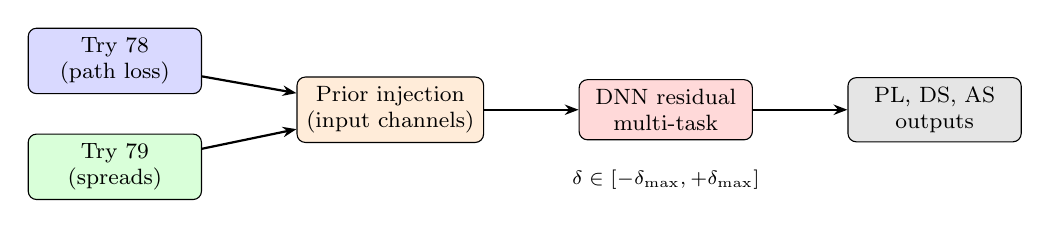
\begin{tikzpicture}[
  box/.style={rectangle, draw, rounded corners=3pt, minimum width=2.2cm,
              minimum height=0.75cm, align=center, font=\footnotesize},
  arr/.style={-{Stealth[length=5pt]}, thick},
  node distance=0.5cm and 1.1cm
]
\node[box, fill=blue!15]  (t78) {Try 78\\(path loss)};
\node[box, fill=green!15, below=of t78] (t79) {Try 79\\(spreads)};
\node[box, fill=orange!15, right=1.2cm of t78, yshift=-0.62cm] (inject)
      {Prior injection\\(input channels)};
\node[box, fill=red!15, right=1.2cm of inject] (dnn)
      {DNN residual\\multi-task};
\node[box, fill=gray!20, right=1.2cm of dnn] (out)
      {PL, DS, AS\\outputs};

\draw[arr] (t78) -- (inject);
\draw[arr] (t79) -- (inject);
\draw[arr] (inject) -- (dnn);
\draw[arr] (dnn) -- (out);

\node[below=0.25cm of dnn, font=\scriptsize, text width=2.4cm, align=center]
      {$\delta \in [-\delta_{\max}, +\delta_{\max}]$};
\end{tikzpicture}
\caption{Overall Try 80 pipeline. The frozen priors from Try 78 and Try 79
are injected as input channels; the deep model predicts bounded residuals on
top of them.}
\label{fig:pipeline}
\end{figure}

%% ============================================================
\section{What was reused from the literature, what was changed, and what is new}
%% ============================================================

This section gives a detailed, item-by-item account of (a) what the literature
provides, (b) what we took from it, (c) what we deliberately changed or did
\emph{not} take, and (d) what is genuinely new in the combination.

\subsection{Try 78: path loss}

\subsubsection{What the literature provides}

\paragraph{Free-space path loss (FSPL).}
FSPL is a textbook formula \cite{rappaport} that gives the power loss of a
plane wave in free space as a function of distance and frequency
(Eq.~\ref{eq:fspl}). It is the universal starting point for any
distance-dependent path-loss model. There is nothing new in using it.

\paragraph{Two-ray / ground-reflection model.}
The two-ray model for a transmitter above a flat reflecting ground is also
classical \cite{rappaport}. For terrestrial base stations, the
``two-ray'' approximation is standard at distances beyond the breakpoint
$d_{\mathrm{bp}} = 4 h_{\mathrm{tx}} h_{\mathrm{rx}} / \lambda$, where the
coherent sum of the two rays simplifies to a $d^{-4}$ power law. For UAV
air-to-ground links at moderate distances, Su et al.\ \cite{wocc2021} and
Khawaja et al.\ \cite{khawaja_survey} both confirm that two-ray behavior is
observable and produces the characteristic ring-like interference pattern.

\paragraph{COST-231 / Hata urban path loss.}
The COST-231 extension of the Hata model is a standard empirical formula for
macrocell path loss in the 1.5--2 GHz range and was later applied at higher
frequencies. It captures the dependence on base-station height, distance, and
urban morphology class. It is used as a coarse NLoS baseline in many
system-level studies.

\paragraph{LoS/NLoS regime separation.}
Treating LoS and NLoS as fundamentally different propagation regimes is a
standard practice in 3GPP TR 38.901 \cite{tr38901}, in UAV channel models
\cite{khawaja_survey}, and in the A2G model family.

\subsubsection{What we took exactly from the literature}

\begin{itemize}
\item The FSPL formula (Eq.~\ref{eq:fspl}) is used verbatim, without any
      modification to the constants or exponents.
\item The two-ray \emph{concept} — direct ray plus ground-reflected ray,
      with a complex-valued sum — is taken directly from the standard derivation
      in \cite{rappaport,wocc2021}.
\item The COST-231 formula (Eq.~\ref{eq:cost231}) is used verbatim, including
      the empirical constants $46.3$, $33.9$, $13.82$, $44.9$, $6.55$, and the
      $+3$ dB metropolitan correction.
\item The qualitative idea of LoS/NLoS regime separation is taken from
      \cite{tr38901,khawaja_survey}.
\end{itemize}

\subsubsection{What we changed or did not take}

\begin{itemize}
\item \textbf{Reflection coefficient $\Gamma$.}
      In the standard two-ray model, $\Gamma$ is computed from Fresnel equations
      for a known ground material (permittivity, conductivity). We do
      \emph{not} use material-based Fresnel coefficients. Instead, $\Gamma$ is
      replaced by an \emph{effective} complex parameter
      $\rho(h_{\mathrm{tx}})\,e^{j\phi(h_{\mathrm{tx}})}$ fitted per UAV
      height bin from data. The motivation is that the ``ground'' in an urban
      CKM map is not a homogeneous flat surface, and the effective reflection
      depends on the mix of buildings, streets, and vegetation visible at each
      UAV height.

\item \textbf{Height-bin fitting instead of a single model.}
      Literature two-ray models are typically written as a single formula for a
      given scenario. Here, independent $(\rho, \phi, b)$ triples are fitted
      per 5 m height bin (Section~\ref{sec:los_calibration}), producing a
      height-dependent effective model. This is necessary because the CKM
      dataset covers a wide range of UAV heights (roughly 10--460 m) and the
      interference geometry changes substantially across that range.

\item \textbf{Radial residual correction.}
      Standard two-ray models do not include a separate range-dependent
      correction term $r(d_{2D})$. We add this because inspection of the CKM
      LoS residuals after the two-ray fit revealed a systematic smooth trend as
      a function of distance, likely caused by the finite urban clutter at
      ground level that the idealized flat-earth two-ray ignores.

\item \textbf{COST-231 application to UAV.}
      The COST-231 model was developed for terrestrial base stations; applying
      it to a UAV that may be 10--400 m above the ground is an extrapolation
      beyond its original validation range. We use it only as a coarse floor
      for the NLoS raw prior (Eq.~\ref{eq:nlos_raw}), combined via $\max$ with
      the A2G envelope. It is never used as the final NLoS prediction on its
      own.

\item \textbf{Regime-wise linear calibration on top of COST-231.}
      The literature does not provide a way to calibrate a coarse formula
      against local building morphology at pixel level. We add the 15-feature
      design vector $X_{78}(x)$ and regime-wise OLS calibration
      (Eq.~\ref{eq:pl_cal}--\ref{eq:ols_closed}) to correct the raw prior
      using density, height, NLoS support, and elevation features derived from
      the CKM map itself. This step has no direct literature equivalent.
\end{itemize}

\subsubsection{What is genuinely new in Try 78}

The contribution of Try 78 is the \emph{combination} and the dataset-driven
calibration, not any individual formula:

\begin{enumerate}
\item fitting an effective two-ray model per height bin from CKM data rather
      than using Fresnel-based material coefficients,
\item adding a smooth radial residual on top of the two-ray fit,
\item building a regime-wise calibrated NLoS model that uses local CKM
      morphology features (density, height, NLoS support) to go beyond what
      COST-231 alone provides,
\item and producing a single hybrid LoS/NLoS path-loss map that is frozen and
      reused as a prior in Try 80.
\end{enumerate}

None of steps 1--4 individually invents a new propagation formula. Each one
adapts a known tool to the CKM pixel-map prediction setting in a way that
is not found as a ready-made combination in any single reference.

\subsection{Try 79: delay spread and angular spread}

\subsubsection{What the literature provides}

\paragraph{Log-normal / log-domain treatment of spreads.}
3GPP TR 38.901 \cite{tr38901} and WINNER II \cite{winner2} model delay spread
and angular spread as log-normal random variables, i.e., their logarithms are
Gaussian. This is empirically well-established across many measurements and
scenarios. The mean of the log-normal varies with distance, height, and
scenario class, and separate parameters are given for LoS and NLoS.

\paragraph{LoS/NLoS and scenario-class conditioning.}
Both 3GPP and WINNER models provide separate tables of spread parameters for
LoS vs.\ NLoS conditions and for different scenario types (urban macro, urban
micro, indoor, suburban, etc.). The LoS/NLoS distinction is fundamental: LoS
channels have smaller, more concentrated angular spreads and shorter delay
spreads because the direct ray dominates.

\paragraph{Distance and elevation-angle dependence.}
Empirical studies on UAV channels \cite{cai2019,izydorczyk2019} report that
delay spread and angular spread increase as the UAV elevation angle decreases
(i.e., at longer horizontal distances), consistent with the UAV seeing more
buildings at shallow angles.

\paragraph{Positive support and right-skewed distributions.}
Both delay spread and angular spread are strictly positive. The literature
universally uses log-domain or log-normal representations because linear-space
Gaussian models would assign probability to negative values.

\subsubsection{What we took exactly from the literature}

\begin{itemize}
\item The log-domain representation: we model $\log(1+y)$ rather than $y$
      directly (Eq.~\ref{eq:log_transform}), in line with 3GPP and WINNER
      practice.
\item The LoS/NLoS separation: different baseline levels and different
      calibrated coefficient vectors per propagation state.
\item The dependence on distance and elevation angle: included as explicit
      terms $\log(1+d_{2D})$ and $\theta_{\mathrm{inv}}$ in both the raw
      prior (Eq.~\ref{eq:raw_spread}) and the design matrix $X_{79}$.
\item The qualitative finding from \cite{cai2019,izydorczyk2019} that
      elevation angle is a key predictor of spread: encoded via
      $\theta_{\mathrm{inv}}$ and its interactions.
\end{itemize}

\subsubsection{What we changed or did not take}

\begin{itemize}
\item \textbf{No stochastic channel simulator.}
      3GPP TR 38.901 and WINNER II provide spread parameters for generating
      random channel realizations per scenario drop. We do \emph{not} generate
      random realizations. Instead, we fit a deterministic regression that
      predicts the \emph{expected} spread value at each map pixel, conditioned
      on the local geometry.

\item \textbf{No generic scenario tables.}
      3GPP gives different tables for UMa, UMi, InH, RMa, etc. We do not
      use those tables directly. The baseline coefficients ($b_{\mathrm{LoS}}$,
      $b_{\mathrm{NLoS}}$, $a_1,\ldots,a_6$ in Eq.~\ref{eq:raw_spread}) are
      set from CKM-specific inspection, not from a 3GPP lookup table.

\item \textbf{Map-derived morphology features.}
      Literature models do not include per-pixel features such as local building
      density $\rho_k(x)$, mean building height $h_k(x)$, NLoS-support fraction
      $n_k(x)$, blocker depth $b_{41}(x)$, transmitter clearance $c_{41}(x)$,
      or taller-building fraction $t_{41}(x)$. These 11 spatial features in
      $X_{79}$ (Eq.~\ref{eq:x79}) are computed directly from the CKM map
      topology tensor and have no equivalent in 3GPP or WINNER.

\item \textbf{Regime-wise ridge regression per pixel.}
      3GPP provides per-scenario stochastic parameters, not per-pixel
      regression coefficients. The regime-wise ridge regression
      (Eq.~\ref{eq:ridge}) and the associated fallback hierarchy are entirely
      our construction, designed to handle the sparse-regime problem that arises
      when the dataset is stratified across
      $\mathrm{metric} \times \mathrm{topology} \times \mathrm{LoS/NLoS} \times
      \mathrm{antenna\_bin}$.

\item \textbf{UAV height as a feature.}
      The normalized height $h_{\mathrm{norm}}$ and its square
      $h_{\mathrm{norm}}^2$ (Eq.~\ref{eq:hnorm}) are included because the CKM
      dataset spans a wide range of UAV heights, and spread varies substantially
      with height. Standard 3GPP models do not include a continuous UAV height
      dimension in this way.
\end{itemize}

\subsubsection{What is genuinely new in Try 79}

\begin{enumerate}
\item Building a raw log-domain prior from simple geometry (distance, elevation
      angle, LoS/NLoS) and then refining it with per-pixel map morphology
      features in a single linear framework.
\item Using a 23-feature design matrix that combines the raw prior, multiscale
      spatial density/height/NLoS features, and the new obstruction/clearance
      features ($b_{41}$, $c_{41}$, $t_{41}$) derived from the CKM topology
      tensor.
\item Fitting regime-wise ridge regression coefficients from the CKM training
      split with incremental sufficient-statistics accumulation, allowing the
      model to scale to the full dataset without ever materializing the full
      design matrix in memory.
\item The fallback hierarchy that gracefully degrades to less specific regimes
      when training data is sparse.
\end{enumerate}

Again, no individual step is a new physical formula. The contribution is the
\emph{pipeline} that maps from a CKM map tensor to a spread prediction map
in a way that is transparent, interpretable, and trainable.

%% ============================================================
\section{Try 78: Path Loss Prior}
%% ============================================================

\subsection{LoS branch: coherent two-ray model}

\subsubsection{Geometry and distances}

Consider a UAV transmitter at height $h_{\mathrm{tx}}$ (metres above the
ground-plane reference) and a receiver at height $h_{\mathrm{rx}}$. For each
map pixel $x$ at 2D horizontal distance $d_{2D}(x)$ from the transmitter, two
propagation distances are defined.

The \emph{direct-path} (LoS) distance is:

\begin{equation}
d_{\mathrm{LoS}}(x)
=
\sqrt{d_{2D}(x)^2 + (h_{\mathrm{tx}} - h_{\mathrm{rx}})^2}
\label{eq:d_los}
\end{equation}

This is simply the Euclidean distance between the two antennas in 3D space.
Because both $d_{2D}(x)$ and the height difference $(h_{\mathrm{tx}} -
h_{\mathrm{rx}})$ are non-negative reals, $d_{\mathrm{LoS}}(x) \ge
d_{2D}(x)$, with equality only when both antennas are at the same height.

The \emph{reflected-path} (image) distance is:

\begin{equation}
d_{\mathrm{ref}}(x)
=
\sqrt{d_{2D}(x)^2 + (h_{\mathrm{tx}} + h_{\mathrm{rx}})^2}
\label{eq:d_ref}
\end{equation}

This is the distance from the image source (the UAV mirrored below the
ground plane at $-h_{\mathrm{tx}}$) to the receiver. Since $(h_{\mathrm{tx}}
+ h_{\mathrm{rx}}) \ge |h_{\mathrm{tx}} - h_{\mathrm{rx}}|$ for any
non-negative heights, we always have $d_{\mathrm{ref}}(x) \ge
d_{\mathrm{LoS}}(x)$, reflecting the fact that the reflected path is always
longer than the direct path.

\begin{figure}[H]
\centering
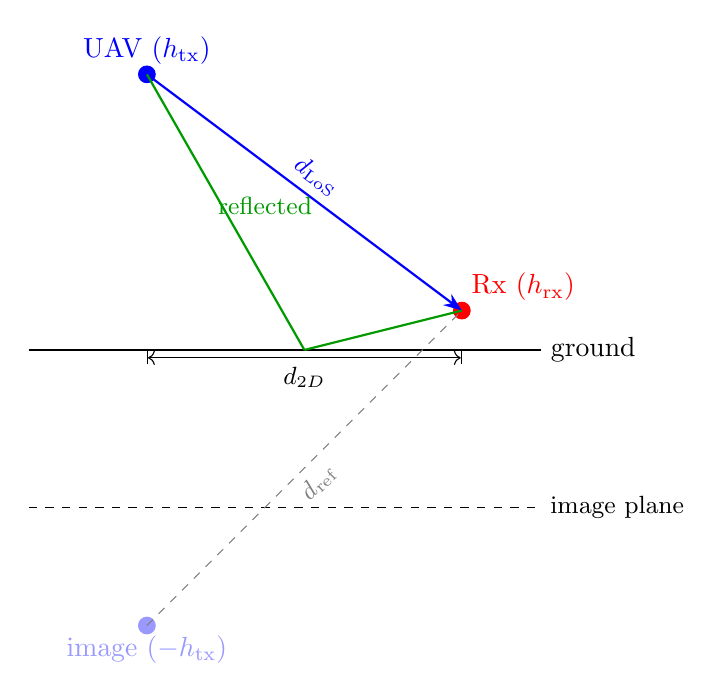
\begin{tikzpicture}[scale=1.0]
\draw[thick] (-0.5,0) -- (6.0,0) node[right] {ground};
\draw[dashed] (-0.5,-2) -- (6.0,-2) node[right, font=\small] {image plane};

\filldraw[blue] (1.0,3.5) circle(3pt) node[above] {UAV ($h_{\mathrm{tx}}$)};
\filldraw[red]  (5.0,0.5) circle(3pt) node[above right] {Rx ($h_{\mathrm{rx}}$)};
\filldraw[blue!40] (1.0,-3.5) circle(3pt) node[below] {image ($-h_{\mathrm{tx}}$)};

\draw[-{Stealth},thick,blue]  (1.0,3.5) -- (5.0,0.5)
      node[midway, above, sloped, font=\small] {$d_{\mathrm{LoS}}$};

\draw[thick,green!60!black] (1.0,3.5) -- (3.0,0.0);
\draw[thick,green!60!black] (3.0,0.0) -- (5.0,0.5);
\node[above, font=\small, green!60!black] at (2.5,1.6) {reflected};

\draw[dashed,gray] (1.0,-3.5) -- (5.0,0.5)
      node[midway, below, sloped, font=\small, gray] {$d_{\mathrm{ref}}$};

\draw[|<->|] (1.0,-0.1) -- (5.0,-0.1) node[midway, below, font=\small] {$d_{2D}$};
\end{tikzpicture}
\caption{Two-ray geometry. Direct path (blue) has length $d_{\mathrm{LoS}}$;
reflected path (green) has the same total length as the image-source path
(gray dashed), which is $d_{\mathrm{ref}}$.}
\label{fig:tworay}
\end{figure}

\subsubsection{Free-space path loss}

The free-space path loss in dB is defined using the standard formula at
frequency $f_{\mathrm{MHz}}$ (in MHz):

\begin{equation}
\mathrm{FSPL}(x)
=
32.45
+ 20 \log_{10}\!\left(\frac{d_{\mathrm{LoS}}(x)}{1000}\right)
+ 20 \log_{10}(f_{\mathrm{MHz}})
\label{eq:fspl}
\end{equation}

\paragraph{Derivation.}
FSPL in linear power ratio is $(4\pi d / \lambda)^2$ where $\lambda = c/f$.
In dB:
\begin{align}
\mathrm{FSPL}_{\mathrm{dB}}
&= 20\log_{10}\!\left(\frac{4\pi d f}{c}\right) \nonumber\\
&= 20\log_{10}(4\pi) + 20\log_{10}(d) + 20\log_{10}(f) - 20\log_{10}(c) \nonumber\\
&\approx 20\log_{10}(d_{\mathrm{km}} \cdot 1000)
  + 20\log_{10}(f_{\mathrm{MHz}} \cdot 10^6) + 20\log_{10}(4\pi) - 20\log_{10}(3\times 10^8) \nonumber\\
&= 20\log_{10}(d_{\mathrm{km}}) + 20\log_{10}(f_{\mathrm{MHz}}) + 32.45 \quad [\mathrm{dB}]
\end{align}

The constant $32.45 = 20\log_{10}(4\pi \cdot 10^3 \cdot 10^6 / (3\times
10^8)) \approx 32.45$ dB. In Eq.~\eqref{eq:fspl}, $d_{\mathrm{LoS}}(x)/1000$
converts metres to kilometres.

\paragraph{Physical meaning.} FSPL grows quadratically with distance ($\propto
d^2$) and quadratically with frequency. It captures only the geometric
spreading of the wavefront, with no ground interaction, scattering, or
diffraction.

\subsubsection{Coherent two-ray correction}

In the two-ray model, the received field is the superposition of the direct
path and a ground-reflected path. Let $k = 2\pi f / c$ be the free-space
wavenumber. The complex sum of the two waves at the receiver is:

\begin{equation}
E_{\mathrm{total}}
\propto
\frac{e^{-jkd_{\mathrm{LoS}}}}{d_{\mathrm{LoS}}}
+
\Gamma\,\frac{e^{-jkd_{\mathrm{ref}}}}{d_{\mathrm{ref}}}
\label{eq:field_sum}
\end{equation}

where $\Gamma$ is the complex ground reflection coefficient. In the standard
textbook derivation, $\Gamma$ is computed from the Fresnel equations for the
ground material. Here, it is replaced by an \emph{effective} complex
parameter:

\begin{equation}
\Gamma(h_{\mathrm{tx}})
=
\rho(h_{\mathrm{tx}})\,e^{j\phi(h_{\mathrm{tx}})}
\end{equation}

where $\rho \in [0, 1.5]$ is the effective amplitude (allowing slight
over-unity to capture constructive multipath effects) and $\phi \in [-\pi,
\pi]$ is the effective phase offset. Both depend on the UAV height bin.

The two-ray path-loss correction term in dB is:

\begin{equation}
C_{\mathrm{2ray}}(x)
=
-20 \log_{10}
\left|
1 + \rho(h_{\mathrm{tx}})
\frac{d_{\mathrm{LoS}}(x)}{d_{\mathrm{ref}}(x)}
e^{-j\left(k\bigl(d_{\mathrm{ref}}(x)-d_{\mathrm{LoS}}(x)\bigr)+\phi(h_{\mathrm{tx}})\right)}
\right|
\label{eq:c2ray}
\end{equation}

\paragraph{Term-by-term interpretation.}
\begin{itemize}
\item $\rho(h_{\mathrm{tx}})$: amplitude of the ground reflection. A value of
      $\rho = 0$ recovers pure FSPL. The fitted values are $\rho \approx
      0.49$--$0.56$ for heights 10--100 m, consistent with a moderate
      ground-reflection coefficient.
\item $d_{\mathrm{LoS}}(x)/d_{\mathrm{ref}}(x)$: path amplitude ratio. This
      is always $\le 1$ since the reflected path is longer; it corrects for
      the $1/d$ amplitude decay of the reflected ray relative to the direct
      ray.
\item $k(d_{\mathrm{ref}}(x) - d_{\mathrm{LoS}}(x))$: the phase difference
      accumulated due to the extra path length of the reflected wave.
\item $\phi(h_{\mathrm{tx}})$: an additional phase offset capturing phase
      shifts upon reflection (e.g., phase shift at the boundary). The fitted
      values are $\phi \approx 0$ for all height bins, meaning in-phase
      reflection dominates.
\item $-20\log_{10}|\cdot|$: the total field amplitude at the receiver,
      normalized to the direct-path field. When the two waves add in phase, the
      field amplitude is $> 1$, giving a \emph{negative} correction (the signal
      is \emph{stronger} than FSPL alone); when they cancel, the correction is
      \emph{positive} (fading loss).
\end{itemize}

This spatial interference pattern creates the characteristic ring-like
behavior in the LoS path-loss maps: concentric rings of constructive and
destructive interference around the transmitter.

\subsubsection{Calibrated LoS prior}

The full calibrated LoS prior is:

\begin{equation}
\mathrm{PL}_{\mathrm{LoS}}(x)
=
\mathrm{FSPL}(x)
+ C_{\mathrm{2ray}}(x)
+ b(h_{\mathrm{tx}})
+ r(d_{2D}(x), h_{\mathrm{tx}})
\label{eq:pl_los}
\end{equation}

where:
\begin{itemize}
\item $b(h_{\mathrm{tx}})$ is a height-dependent bias (dB): a constant
      correction that shifts the overall two-ray prediction for a given UAV
      height.
\item $r(d_{2D}(x), h_{\mathrm{tx}})$ is a radial residual correction: a
      smooth function of horizontal distance (and height bin) that captures
      systematic over-/under-prediction of the two-ray model as a function of
      range. It is obtained by smoothing the empirical mean residual in each
      distance bin after the two-ray fit.
\end{itemize}

The four terms in Eq.~\eqref{eq:pl_los} are applied sequentially:
FSPL gives the geometric baseline; the two-ray correction adds the
interference pattern; the bias corrects for a systematic global offset per
height; and the radial term corrects for range-dependent systematic errors.

\subsection{Calibration of the LoS two-ray model}
\label{sec:los_calibration}

\subsubsection{Data preparation}

All training samples are used. For each sample, valid LoS pixels are selected
as those satisfying:
\begin{enumerate}
\item topology label = 0 (ground pixel),
\item $m_{\mathrm{LoS}}(x) > 0$ (marked as LoS),
\item the measured path loss is finite and $\ge 20$ dB.
\end{enumerate}
If a sample has more than 2\,500 valid LoS pixels, a random subsample of
2\,500 pixels is drawn (with a fixed seed). Samples are then grouped by UAV
height into height bins of 5 m width:

\begin{equation}
h_{\mathrm{bin}} = 5 \cdot \left\lfloor \frac{h_{\mathrm{tx}}}{5} \right\rceil
\end{equation}

Each bin is further subsampled to a maximum of 8\,000 pixels total.

\subsubsection{Grid search for $(\rho, \phi)$}

For each height bin, $(\rho, \phi)$ are found by grid search:

\begin{align}
\phi_{\mathrm{grid}} &= \left\{-\pi + \frac{2\pi k}{N_\phi} : k = 0, 1, \ldots, N_\phi - 1\right\},
\quad N_\phi = 48 \label{eq:phi_grid}\\
\rho_{\mathrm{grid}} &= \{0.00,\, 0.05,\, 0.10,\, \ldots,\, 1.50\}
\label{eq:rho_grid}
\end{align}

For each pair $(\hat\rho, \hat\phi) \in \rho_{\mathrm{grid}} \times
\phi_{\mathrm{grid}}$, and for each pixel $x_i$ in the height bin, define
the two-ray prediction without bias:

\begin{equation}
\hat p_i(\hat\rho, \hat\phi)
=
\mathrm{FSPL}(x_i)
- 20\log_{10}
\left|
1 + \hat\rho\,\frac{d_{\mathrm{LoS}}(x_i)}{d_{\mathrm{ref}}(x_i)}
e^{-j\left(k(d_{\mathrm{ref}}-d_{\mathrm{LoS}})+\hat\phi\right)}
\right|
\end{equation}

The optimal bias for each $(\hat\rho, \hat\phi)$ pair is solved analytically
as the empirical mean of residuals:

\begin{equation}
\hat b(\hat\rho, \hat\phi)
=
\frac{1}{N}\sum_{i=1}^{N}
\left(y_i - \hat p_i(\hat\rho, \hat\phi)\right)
\end{equation}

where $y_i$ is the measured path loss at pixel $x_i$ and $N$ is the number
of pixels in the bin. The biased prediction is $\hat p_i + \hat b$, and the
RMSE for the pair is:

\begin{equation}
\mathrm{RMSE}(\hat\rho, \hat\phi)
=
\sqrt{\frac{1}{N}\sum_{i=1}^{N}
\left(y_i - \hat p_i(\hat\rho,\hat\phi) - \hat b(\hat\rho,\hat\phi)\right)^2}
\label{eq:rmse_grid}
\end{equation}

The best pair is:

\begin{equation}
(\rho^*, \phi^*)
= \arg\min_{(\hat\rho, \hat\phi)}
\mathrm{RMSE}(\hat\rho, \hat\phi)
\end{equation}

\subsubsection{Post-fit Gaussian smoothing across height bins}

After fitting all bins independently, a Gaussian-weighted smooth is applied
to stabilize sparse high-altitude bins. Let $\{h_k\}$ be the fitted height
bin centers, $\{(\rho_k^*, b_k^*)\}$ the per-bin fitted values, and $\{N_k\}$
the pixel counts used in fitting. The smoothed values are:

\begin{equation}
\tilde\rho(h)
=
\frac{\sum_k w_k(h)\,N_k\,\rho_k^*}{\sum_k w_k(h)\,N_k},
\qquad
w_k(h) = \exp\!\left(-\frac{(h - h_k)^2}{2\sigma_h^2}\right),
\quad \sigma_h = 10\;\mathrm{m}
\label{eq:gauss_smooth}
\end{equation}

and similarly for $b$. The phase $\phi$ is always replaced with its smoothed
version (treating it as effectively constant across heights).

Bins where both $\rho_k^*$ and $b_k^*$ differ noticeably from the smoothed
global trend are flagged as suspicious (typically high-altitude bins with few
samples), and their raw fit values are replaced by the smoothed values.

\subsubsection{Radial residual correction}

After fitting the two-ray model, a residual correction is computed:

\begin{equation}
r(d_{2D}) =
\mathrm{GaussSmooth}_{\sigma_r}\left(
\mathrm{clip}\left(
\mu_{\Delta}(d_{2D}),\, -2.5,\, +2.5
\right)
\right)
\end{equation}

where $\mu_{\Delta}(d_{2D})$ is the empirical mean of $(y - \hat y_{\mathrm{2ray}})$
averaged over all pixels at horizontal distance $d_{2D}$, $\sigma_r = 1.5$
pixels is a Gaussian smoothing radius, and clipping limits the correction to
$\pm 2.5$ dB to prevent over-fitting on noisy radius bins.

\subsubsection{Fitted parameter values}

Table~\ref{tab:los_params} shows representative fitted LoS two-ray parameters
across height bins.

\begin{table}[H]
\centering
\caption{Representative fitted LoS two-ray parameters by height bin.}
\label{tab:los_params}
\small
\begin{tabular}{rrrr}
\toprule
$h_{\mathrm{tx}}$ (m) & $\rho^*$ & $\phi^*$ (rad) & $b^*$ (dB)\\
\midrule
10  & 0.5605 & 0.000 & $-$0.037 \\
20  & 0.5242 & 0.000 & $-$0.042 \\
30  & 0.4950 & 0.000 & $-$0.046 \\
50  & 0.5468 & 0.000 & $-$0.014 \\
80  & 0.5482 & 0.000 & $-$0.027 \\
100 & 0.5463 & 0.000 & $-$0.017 \\
140 & 0.5414 & 0.000 & $+$0.255 \\
200 & 0.5435 & 0.000 & $+$0.561 \\
460 & 0.8966 & $-$0.047 & $+$1.521 \\
\bottomrule
\end{tabular}
\end{table}

The dominant pattern is $\rho \approx 0.49$--$0.56$ with $\phi \approx 0$
for heights 10--100 m, meaning a moderate-amplitude in-phase ground
reflection. Biases are near-zero ($< 0.05$ dB) for these bins. At very high
altitudes ($>140$ m), the increasing positive bias and higher $\rho$ values
reflect sparser training data; those bins are stabilized by Gaussian
smoothing.

\begin{figure}[H]
\centering
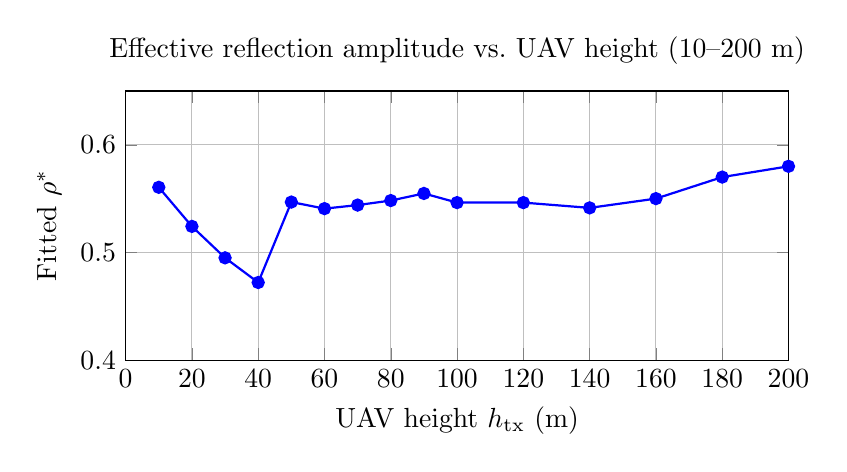
\begin{tikzpicture}
\begin{axis}[
  width=10cm, height=5cm,
  xlabel={UAV height $h_{\mathrm{tx}}$ (m)},
  ylabel={Fitted $\rho^*$},
  xmin=0, xmax=200,
  ymin=0.4, ymax=0.65,
  grid=major,
  title={Effective reflection amplitude vs.\ UAV height (10--200 m)}
]
\addplot[mark=*, thick, blue] coordinates {
  (10,0.5605)(20,0.5242)(30,0.4950)(40,0.4721)
  (50,0.5468)(60,0.5407)(70,0.5440)(80,0.5482)
  (90,0.5548)(100,0.5463)(120,0.5463)(140,0.5414)
  (160,0.55)(180,0.57)(200,0.58)
};
\end{axis}
\end{tikzpicture}
\caption{Effective ground-reflection amplitude $\rho^*$ as a function of UAV
height, fitted independently per 5 m height bin. Values are stable in the
range $0.47$--$0.56$ for 10--130 m, then rise slightly at higher altitudes
where training data is sparser.}
\label{fig:rho_vs_h}
\end{figure}

\begin{figure}[H]
\centering
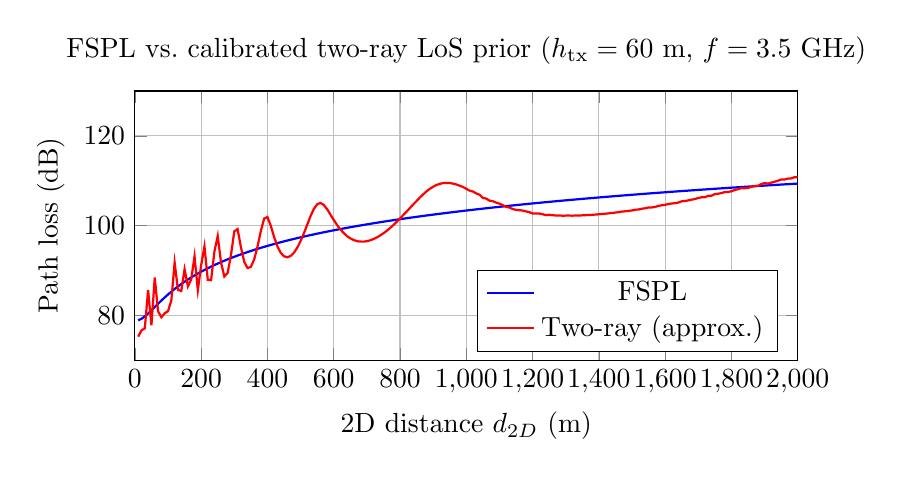
\begin{tikzpicture}
\begin{axis}[
  width=10cm, height=5cm,
  xlabel={2D distance $d_{2D}$ (m)},
  ylabel={Path loss (dB)},
  xmin=0, xmax=2000,
  ymin=70, ymax=130,
  grid=major,
  legend pos=south east,
  title={FSPL vs.\ calibrated two-ray LoS prior ($h_{\mathrm{tx}} = 60$ m, $f = 3.5$ GHz)}
]
\addplot[thick, blue, domain=10:2000, samples=200]
  {32.45 + 20*ln(sqrt(x^2+3481)/1000)/ln(10) + 20*ln(3500)/ln(10)};
\addlegendentry{FSPL}
\addplot[thick, red, domain=10:2000, samples=200]
  {32.45 + 20*ln(sqrt(x^2+3481)/1000)/ln(10) + 20*ln(3500)/ln(10)
   - 20*ln(abs(1 + 0.54 * sqrt(x^2+3481)/sqrt(x^2+3721) *
   cos(deg(2*3.14159*(sqrt(x^2+3721)-sqrt(x^2+3481))*3500e6/3e8))))/ln(10)};
\addlegendentry{Two-ray (approx.)}
\end{axis}
\end{tikzpicture}
\caption{Schematic comparison of FSPL and the coherent two-ray model for a
60 m UAV at 3.5 GHz ($h_{\mathrm{rx}} = 1.5$ m). The two-ray model produces
a characteristic oscillatory pattern around the FSPL baseline, corresponding
to alternating zones of constructive and destructive interference.}
\label{fig:tworay_pl}
\end{figure}

\subsection{NLoS branch}
\label{sec:nlos_branch}

The NLoS path-loss branch used in \texttt{Try 80} is not a pure literature
formula. It is a hybrid engineering model built in four stages.

\subsubsection{Stage 1: raw NLoS propagation prior}

Two coarse physical estimates are combined.

\paragraph{COST-231 term.}
The COST-231 / Hata extension for urban macro cells gives:

\begin{equation}
\mathrm{PL}_{\mathrm{COST231}}(x)
=
46.3 + 33.9 \log_{10}(f_{\mathrm{MHz}})
- 13.82 \log_{10}(h_{\mathrm{tx}})
- a(h_{\mathrm{rx}})
+ \left(44.9 - 6.55 \log_{10}(h_{\mathrm{tx}})\right)\log_{10}(d_{\mathrm{km}})
+ 3
\label{eq:cost231}
\end{equation}

where $d_{\mathrm{km}} = d_{2D}(x)/1000$ and the mobile antenna correction
factor for large cities is:

\begin{equation}
a(h_{\mathrm{rx}}) = 3.2(\log_{10}(11.75\,h_{\mathrm{rx}}))^2 - 4.97
\label{eq:cost231_a}
\end{equation}

\paragraph{Interpretation of Eq.~\eqref{eq:cost231}.}
\begin{itemize}
\item $46.3 + 33.9\log_{10}(f_{\mathrm{MHz}})$: frequency-dependent offset.
      The exponent $33.9$ (compare to $20$ for FSPL) reflects stronger
      frequency dependence in urban scattering.
\item $-13.82\log_{10}(h_{\mathrm{tx}})$: as the base station / UAV gets
      higher, path loss decreases (better clearance above rooftops). The
      $-13.82$ coefficient is a fitted constant from the Hata empirical
      dataset.
\item $-a(h_{\mathrm{rx}})$: accounts for the receiver height. For typical
      pedestrian heights ($h_{\mathrm{rx}} \approx 1.5$ m), $a \approx
      -0.6$ dB, which is small.
\item $(44.9 - 6.55\log_{10}(h_{\mathrm{tx}}))\log_{10}(d_{\mathrm{km}})$:
      distance-dependent term. The effective path-loss exponent is
      $(44.9 - 6.55\log_{10}(h_{\mathrm{tx}}))/10$, which decreases as the
      UAV climbs (effectively reducing NLoS scattering losses at longer
      distances from higher altitudes).
\item $+3$: the COST-231 metropolitan correction constant (dB).
\end{itemize}

\paragraph{Elevation-aware UAV envelope.}
The A2G NLoS envelope models the elevation-angle dependence of urban air-to-ground path loss:

\begin{equation}
\mathrm{PL}_{\mathrm{A2G,NLoS}}(x)
=
\lambda_0(h_{\mathrm{tx}}, f)
+ \beta_{\mathrm{NLoS}}
+ A_{\mathrm{NLoS}}
\exp\!\left(-\frac{90-\theta^\circ(x)}{\tau_{\mathrm{NLoS}}}\right)
\label{eq:a2g_nlos}
\end{equation}

where:
\begin{align}
\lambda_0(h_{\mathrm{tx}}, f)
&= 20\log_{10}\!\left(\frac{4\pi h_{\mathrm{tx}} f}{c}\right)
\label{eq:lambda0}
\end{align}

The fitted constants are:
$\beta_{\mathrm{NLoS}} = -16.16$ dB,
$A_{\mathrm{NLoS}} = 12.0436$,
$\tau_{\mathrm{NLoS}} = 7.52$ deg.

\paragraph{Interpretation of Eq.~\eqref{eq:a2g_nlos}.}
\begin{itemize}
\item $\lambda_0$: a free-space-like offset that scales with UAV height and
      frequency~\cite{khawaja_survey,wocc2021}. The CKM dataset uses
      $f = 7.125$ GHz (FR3 6G frequency band); for
      $h_{\mathrm{tx}} = 50$ m at that frequency, $\lambda_0 \approx 103$ dB.
\item $\beta_{\mathrm{NLoS}} = -16.16$ dB: a baseline NLoS attenuation
      offset relative to $\lambda_0$.
\item $A_{\mathrm{NLoS}}\exp(-\ldots)$: an exponential modulation with
      $(90 - \theta^\circ)$. When the elevation angle $\theta^\circ$ is high
      (UAV nearly overhead, $\theta^\circ \to 90^\circ$), the exponent
      vanishes and the term goes to $A_{\mathrm{NLoS}}$. When $\theta^\circ$
      is low (grazing incidence), the exponent is large and the term
      approaches zero. The effect is that NLoS path loss \emph{decreases} as
      the UAV moves overhead, consistent with improved clearance above
      buildings.
\item $\tau_{\mathrm{NLoS}} = 7.52^\circ$: the characteristic angular scale.
      A low value means the transition from grazing to overhead happens
      sharply within a small elevation range.
\end{itemize}

The raw NLoS prior is then the conservative (higher) of the two estimates:

\begin{equation}
\mathrm{PL}_{\mathrm{NLoS,raw}}(x)
=
\max\left(
\mathrm{PL}_{\mathrm{COST231}}(x),
\mathrm{PL}_{\mathrm{A2G,NLoS}}(x)
\right)
\label{eq:nlos_raw}
\end{equation}

The full raw prior blends the LoS and NLoS estimates using the LoS mask
$m_{\mathrm{LoS}}(x) \in [0,1]$:

\begin{equation}
\mathrm{PL}^{(0)}(x)
=
m_{\mathrm{LoS}}(x)\,\mathrm{PL}_{\mathrm{LoS,blend}}(x)
+
\left(1-m_{\mathrm{LoS}}(x)\right)\mathrm{PL}_{\mathrm{NLoS,raw}}(x)
\label{eq:pl0}
\end{equation}

with a soft blend for the LoS branch:

\begin{equation}
\mathrm{PL}_{\mathrm{LoS,blend}}(x)
=
0.7\,\mathrm{PL}_{\mathrm{LoS,path}}(x)
+0.3\min\left(\mathrm{PL}_{\mathrm{LoS,path}}(x), \mathrm{PL}_{\mathrm{A2G,LoS}}(x)\right)
\label{eq:los_blend}
\end{equation}

The $0.7/0.3$ blend in Eq.~\eqref{eq:los_blend} gives 70\% weight to the
two-ray LoS model and 30\% weight to the minimum of the two-ray model and an
A2G LoS envelope. This prevents the prediction from exceeding a physically
motivated upper bound in the LoS case.

\subsubsection{Stage 2: map-derived morphology features}

From $\mathrm{PL}^{(0)}(x)$ and the map topology, a 15-element feature
vector is computed:

\begin{equation}
X_{78}(x)
=
\begin{bmatrix}
\mathrm{PL}^{(0)}(x)^2 \\
\mathrm{PL}^{(0)}(x) \\
\log(1+d_{2D}(x)) \\
\rho_{15}(x) \\
\rho_{41}(x) \\
h_{15}(x) \\
h_{41}(x) \\
\rho_{41}(x)\log(1+d_{2D}(x)) \\
n_{15}(x) \\
n_{41}(x) \\
n_{41}(x)\log(1+d_{2D}(x)) \\
\sigma_{\mathrm{shadow}}(x) \\
\theta_{\mathrm{norm}}(x) \\
n_{41}(x)\theta_{\mathrm{norm}}(x) \\
1
\end{bmatrix}
\label{eq:x78}
\end{equation}

Each term is now described in detail.

\paragraph{Base masks.}
The ground mask is:

\begin{equation}
g(x)=
\begin{cases}
1, & \text{if } \mathrm{topology}(x)=0 \\
0, & \text{otherwise}
\end{cases}
\label{eq:ground_mask}
\end{equation}

The building mask is $b(x)=1-g(x)$.
The ground-NLoS support mask is:

\begin{equation}
n_{\mathrm{raw}}(x)=
\mathbf{1}\!\left[m_{\mathrm{LoS}}(x)\le 0.5\right]\cdot g(x)
\label{eq:nlos_mask}
\end{equation}

This selects ground pixels that are predominantly in NLoS, i.e., pixels that
are at street level and are shielded from the UAV.

\paragraph{Quadratic raw-prior feature.}
The pair $(\mathrm{PL}^{(0)}(x)^2, \mathrm{PL}^{(0)}(x))$ allows the linear
model to fit a \emph{quadratic} relationship in the raw prior. Including both
$P^2$ and $P$ as features lets the calibration curve be:
$\hat P = \beta_1 P^2 + \beta_2 P + \cdots$, which can correct for
systematic curvature in the raw prior.

\paragraph{Distance term.}
$\log(1+d_{2D}(x))$: the logarithm of one plus the horizontal distance,
providing a distance-dependent offset. The $+1$ prevents a singularity at
$d_{2D}=0$.

\paragraph{Per-pixel box-mean operator.}
\label{par:boxmean}

All multiscale features use the same 2D box-mean operator
$\mathrm{BoxMean}_k$. For a map $f : \mathbb{Z}^2 \to \mathbb{R}$ and a
window half-width $p = \lfloor k/2 \rfloor$, the value at pixel
$x = (i, j)$ is:

\begin{equation}
\mathrm{BoxMean}_k(f)(i,j)
=
\frac{1}{k^2}
\sum_{i'=i-p}^{i+p}\,\sum_{j'=j-p}^{j+p}
f_{\mathrm{padded}}(i',j')
\label{eq:boxmean}
\end{equation}

where $f_{\mathrm{padded}}$ is $f$ extended outside the map boundary by
\emph{reflect} (mirror) padding: $f_{\mathrm{padded}}(-r, j) =
f_{\mathrm{padded}}(r, j)$ and similarly at all four edges. This ensures
border pixels receive a full $k^2$-pixel average, with the map reflected back
inward rather than zero-padded.

Equation~\eqref{eq:boxmean} is evaluated efficiently using a
\emph{2D summed-area table} (integral image). Let $I(i,j)=\sum_{i'\le
i, j'\le j} f_{\mathrm{padded}}(i',j')$ be the prefix-sum array. Then:

\begin{equation}
\sum_{i'=i-p}^{i+p}\sum_{j'=j-p}^{j+p} f_{\mathrm{padded}}(i',j')
=
I(i+p,\,j+p)
-I(i-p-1,\,j+p)
-I(i+p,\,j-p-1)
+I(i-p-1,\,j-p-1)
\label{eq:sat}
\end{equation}

This reduces each per-pixel evaluation to four table lookups, making the
full-map computation $O(HW)$ regardless of $k$. In the implementation,
$k \in \{15, 41\}$ pixels, corresponding to $\sim$15 m and $\sim$41 m
neighborhoods (1 m/pixel resolution).

\paragraph{Multiscale building density.}

\begin{equation}
\rho_k(x)=\mathrm{BoxMean}_k\!\left(b(\cdot)\right)(x)
=
\frac{1}{k^2}\sum_{x' \in W_k(x)} b(x')
\label{eq:rho_k}
\end{equation}

where $W_k(x)$ is the $k\times k$ window centered at $x$.
Since $b(x') \in \{0,1\}$, $\rho_k(x)$ is the \emph{fraction of pixels
that are buildings} in the window. It is zero at a ground pixel
surrounded only by other ground pixels, and one at a pixel deep inside a
solid building block. $\rho_{15}$ captures fine-scale building density within
a $\sim$15 m neighborhood; $\rho_{41}$ captures a coarser $\sim$41 m
neighborhood.

\paragraph{Multiscale building height.}

\begin{equation}
h_k(x)=
\frac{\mathrm{BoxMean}_k\!\left(\mathrm{topology}(\cdot)\,b(\cdot)\right)(x)}
{H_{\mathrm{norm}}},
\quad H_{\mathrm{norm}} = 90 \;\mathrm{m}
\label{eq:h_k}
\end{equation}

This is the box mean of $\mathrm{topology}(x')\cdot b(x')$:
building pixels contribute their height in metres; ground pixels contribute
0. Dividing by $k^2$ (inside $\mathrm{BoxMean}_k$) gives:

\begin{equation}
h_k(x)=
\frac{1}{H_{\mathrm{norm}}\,k^2}
\sum_{x'\in W_k(x)}
\mathrm{topology}(x')\cdot b(x')
=
\frac{\rho_k(x)}{H_{\mathrm{norm}}}\;\overline{h}_{\mathrm{bldg},k}(x)
\label{eq:h_k_interp}
\end{equation}

where $\overline{h}_{\mathrm{bldg},k}(x)$ is the \emph{mean height of
building pixels only} within the window:

\begin{equation}
\overline{h}_{\mathrm{bldg},k}(x)
=
\frac{\displaystyle\sum_{x'\in W_k(x)} \mathrm{topology}(x')\,b(x')}
     {\displaystyle\sum_{x'\in W_k(x)} b(x')}
\quad\text{(undefined if }\rho_k(x)=0\text{)}
\label{eq:mean_bldg_height}
\end{equation}

Critically, $h_k(x) = \rho_k(x)\cdot\overline{h}_{\mathrm{bldg},k}(x)/H_{\mathrm{norm}}$,
so $h_k$ combines \emph{both} how many buildings are present and how tall they
are. A window with 50\% building coverage and mean height 20 m gives the same
$h_k$ as a window with 100\% coverage at mean height 10 m. The $H_{\mathrm{norm}}
= 90$ m normalizer maps the joint range to approximately $[0, 1]$.

\paragraph{Multiscale NLoS-support.}

\begin{equation}
n_k(x)=\mathrm{BoxMean}_k\!\left(n_{\mathrm{raw}}(\cdot)\right)(x)
\label{eq:n_k}
\end{equation}

Since $n_{\mathrm{raw}}(x') \in \{0,1\}$ (Eq.~\ref{eq:nlos_mask}),
$n_k(x)$ is the \emph{absolute fraction of the window area} that consists of
ground pixels in NLoS. Just as $h_k(x)$ conflates building coverage and building
height, $n_k(x)$ conflates ground coverage and NLoS probability. We can write:

\begin{equation}
n_k(x)
=
\left(1 - \rho_k(x)\right)
\overline{n}_{\mathrm{ground}, k}(x)
\label{eq:n_k_interp}
\end{equation}

where $\overline{n}_{\mathrm{ground}, k}(x)$ is the relative fraction of
\emph{available ground pixels} that are shielded:

\begin{equation}
\overline{n}_{\mathrm{ground}, k}(x)
=
\frac{\displaystyle\sum_{x'\in W_k(x)} n_{\mathrm{raw}}(x')}
     {\displaystyle\sum_{x'\in W_k(x)} g(x')}
\quad\text{(undefined if }\rho_k(x)=1\text{)}
\end{equation}

Because building pixels never contribute to $n_k$, this feature is zero in
completely open LoS areas (where $\overline{n}_{\mathrm{ground}, k} = 0$)
\emph{and} deep inside solid building blocks (where $1 - \rho_k = 0$). It
reaches its maximum in narrow urban street canyons, where ground coverage is
still significant but entirely shielded from the UAV.

\paragraph{Elevation angle.}

\begin{equation}
\theta(x)=\arctan\left(\frac{h_{\mathrm{tx}}-h_{\mathrm{rx}}}{\max(d_{2D}(x),1)}\right)
\label{eq:theta}
\end{equation}

The $\max(\cdot, 1)$ prevents division by zero directly below the UAV.
Then:

\begin{equation}
\theta_{\mathrm{norm}}(x)=
\mathrm{clip}\left(\frac{\theta^\circ(x)}{90},\,0,\,1\right)
\label{eq:theta_norm}
\end{equation}

where $\theta^\circ = \theta \cdot 180/\pi$ is in degrees. $\theta_{\mathrm{norm}}
= 0$ at grazing incidence, $= 1$ directly overhead.

\paragraph{Shadowing proxy.}

\begin{align}
\sigma_{\mathrm{LoS}}(x) &= \alpha_{\mathrm{LoS}}\,(90-\theta^\circ(x))^{\mu_{\mathrm{LoS}}}
\label{eq:sigma_los}\\
\sigma_{\mathrm{NLoS}}(x) &= \alpha_{\mathrm{NLoS}}\,(90-\theta^\circ(x))^{\mu_{\mathrm{NLoS}}}
\label{eq:sigma_nlos}
\end{align}

with fitted values $\alpha_{\mathrm{NLoS}} = 2.3197$, $\mu_{\mathrm{NLoS}}
= 0.2361$. The blended proxy is:

\begin{equation}
\sigma_{\mathrm{shadow}}(x)=
m_{\mathrm{LoS}}(x)\,\sigma_{\mathrm{LoS}}(x)
+\left(1-m_{\mathrm{LoS}}(x)\right)\sigma_{\mathrm{NLoS}}(x)
\label{eq:sigma_blend}
\end{equation}

This acts as a spatially varying uncertainty proxy: higher values at low
elevation angles, where propagation conditions are more difficult.

\paragraph{Interaction terms.}
The three pairwise products
$\rho_{41}(x)\log(1+d_{2D}(x))$,
$n_{41}(x)\log(1+d_{2D}(x))$, and
$n_{41}(x)\theta_{\mathrm{norm}}(x)$
allow the linear model to capture effects where building density or NLoS
support \emph{modifies} the slope of path loss with distance or elevation
angle, rather than just shifting it.

\subsubsection{Stage 3: regime-wise linear calibration}

The regime $r$ is identified by three keys:
\begin{itemize}
\item \emph{Coarse topology:} one of \texttt{open\_lowrise},
      \texttt{mixed\_midrise}, or \texttt{dense\_highrise},
\item \emph{Propagation state:} \texttt{LoS} or \texttt{NLoS},
\item \emph{Antenna height bin:} \texttt{low\_ant}, \texttt{mid\_ant}, or
      \texttt{high\_ant}.
\end{itemize}
This gives up to $3 \times 2 \times 3 = 18$ regimes.

\paragraph{How topology class and antenna bin are computed.}
These are \emph{per-map} scalar labels, not per-pixel quantities.
They are derived once from the full topology tensor and UAV height.

The \emph{map-level} building density and mean building height are:

\begin{align}
\bar\rho_{\mathrm{map}}
&= \frac{1}{HW}\sum_{x} b(x)
\label{eq:global_density}\\[4pt]
\bar h_{\mathrm{map}}
&= \frac{\displaystyle\sum_{x} \mathrm{topology}(x)\,b(x)}
        {\displaystyle\sum_{x} b(x)}
\label{eq:global_mean_bldg_height}
\end{align}

$\bar\rho_{\mathrm{map}}$ is simply the fraction of map pixels that are
buildings. $\bar h_{\mathrm{map}}$ is the mean building height
\emph{over building pixels only} (the denominator excludes ground pixels).
This is different from the per-pixel feature $h_k(x)$ in
Eq.~\eqref{eq:h_k_interp}, which divides the same numerator by the full
window area $k^2$ instead of by the number of building pixels.

The six topology classes are assigned by thresholding both quantities:

\begin{equation}
\mathrm{class}_6 =
\begin{cases}
\texttt{open\_sparse\_lowrise}   & \bar\rho \le d_1,\; \bar h \le h_1 \\
\texttt{open\_sparse\_vertical}  & \bar\rho \le d_1,\; \bar h > h_1 \\
\texttt{dense\_block\_midrise}   & \bar\rho \ge d_2,\; \bar h \le h_2 \\
\texttt{dense\_block\_highrise}  & \bar\rho \ge d_2,\; \bar h > h_2 \\
\texttt{mixed\_compact\_lowrise} & d_1 < \bar\rho < d_2,\; \bar h \le h_1 \\
\texttt{mixed\_compact\_midrise} & d_1 < \bar\rho < d_2,\; \bar h > h_1
\end{cases}
\label{eq:topo6}
\end{equation}

with thresholds $d_1 = 0.12$, $d_2 = 0.28$ (density fractions),
$h_1 = 12$ m, $h_2 = 28$ m. The three-class label
(\texttt{open}/\texttt{mixed}/\texttt{dense}) is the prefix of
$\mathrm{class}_6$ and is used in \texttt{Try 80} reporting.

The antenna-height bin is assigned by UAV height tertiles:

\begin{equation}
\mathrm{ant\_bin} =
\begin{cases}
\texttt{low\_ant}  & h_{\mathrm{tx}} \le 58.12\;\mathrm{m} \\
\texttt{mid\_ant}  & 58.12 < h_{\mathrm{tx}} \le 103.85\;\mathrm{m} \\
\texttt{high\_ant} & h_{\mathrm{tx}} > 103.85\;\mathrm{m}
\end{cases}
\label{eq:ant_bin}
\end{equation}

The calibrated prediction for regime $r$ is:
\begin{equation}
\widehat{\mathrm{PL}}_{r}(x)
=
X_{78}(x)^\top \beta^{78}_{r}
=
\sum_{j=1}^{15} x_j(x)\,\beta^{78}_{r,j}
\label{eq:pl_cal}
\end{equation}

\paragraph{How $\beta^{78}_{r}$ is fitted.}
Across all training samples whose regime label equals $r$, a linear
regression is run:

\begin{equation}
\hat\beta^{78}_{r}
=
\arg\min_\beta \sum_{x \in \mathcal{S}_r} \left(y(x) - X_{78}(x)^\top \beta\right)^2
\label{eq:ols}
\end{equation}

where $\mathcal{S}_r$ is the set of all valid pixels in training samples
belonging to regime $r$. This ordinary least squares problem has the closed
form solution:

\begin{equation}
\hat\beta^{78}_{r}
=
\left(\mathbf{X}_r^\top \mathbf{X}_r\right)^{-1}
\mathbf{X}_r^\top \mathbf{y}_r
\label{eq:ols_closed}
\end{equation}

where $\mathbf{X}_r$ stacks the feature vectors and $\mathbf{y}_r$ stacks
the measured path-loss values. In practice, if the matrix is near-singular
(sparse regime), a fallback to a less specific regime key is used (see
the fallback chain in the Try 79 section, which uses the same strategy).

An example fitted coefficient vector for the \texttt{mixed\_midrise|LoS|high\_ant}
regime is:
\[
\beta^{78}_{\texttt{mixed|LoS|high}}
=
\begin{bmatrix}
-0.000554,\ 0.761,\ 3.061,\ 0.127,\ 0.793,\ -2.318,\ -0.481,\ -0.157 \\[4pt]
0.155,\ -0.218,\ 0.060,\ -47.15,\ -28.08,\ -0.508,\ 48.83
\end{bmatrix}^\top
\]
The large bias weight ($\beta_{15} = 48.83$) and the large negative
shadowing-proxy weight ($\beta_{12} = -47.15$) partially cancel, together
acting as a calibrated effective offset for this regime.

\subsubsection{Stage 4: region replacement and clipping}

\begin{equation}
\mathrm{PL}_{\mathrm{NLoS}}(x)
=
\mathrm{clip}\!\left(
X_{78}(x)^\top \beta^{78}_{r},
20,
180
\right)
\label{eq:pl_nlos_final}
\end{equation}

Hard clipping to $[20, 180]$ dB prevents the linear model from producing
physically unreasonable values. The final hybrid path-loss prior is:

\begin{equation}
\mathrm{PL}_{\mathrm{prior}}(x)
=
\begin{cases}
\mathrm{PL}_{\mathrm{LoS}}(x), & m_{\mathrm{LoS}}(x) > 0.5 \\
\mathrm{PL}_{\mathrm{NLoS}}(x), & \text{otherwise}
\end{cases}
\label{eq:pl_hybrid}
\end{equation}

\subsection{Evaluation metric: pixel-weighted RMSE}

\label{sec:pw_metric}

All numerical results are reported as \emph{pixel-weighted} (pw) RMSE or MAE.
Building pixels ($\mathrm{topology}(x) > 0$) are always excluded; only valid
ground pixels with a finite, physically plausible target value contribute.
Let $\mathcal{V}_k$ be the set of all such valid $(s, x)$ pairs across all
evaluation samples for task $k$. Then:

\begin{equation}
\mathrm{RMSE}^{\mathrm{pw}}_k
=
\sqrt{
  \frac{\displaystyle\sum_{(s,x)\in\mathcal{V}_k}
  \left(\hat{y}_k^{(s)}(x) - y_k^{(s)}(x)\right)^2}
  {\displaystyle|\mathcal{V}_k|}
}
\label{eq:rmse_pw}
\end{equation}

This is a single square root over all pooled valid pixels, not an average of
per-sample RMSEs. Units are dB (path loss), ns (delay spread), and
degrees (angular spread), all in the native non-transformed domain.

\subsection{Observed Try 78 results}

Table~\ref{tab:try78_rmse} summarizes the path-loss RMSE values obtained from
the final hybrid evaluation.

\begin{table}[H]
\centering
\caption{Try 78 pixel-weighted RMSE (dB) on the evaluation split. The
``Role'' column indicates whether the model is used as a frozen prior in
\texttt{Try 80}, serves only as an ablation baseline, or is an intermediate
construction step.}
\label{tab:try78_rmse}
\begin{tabular}{lcc}
\toprule
Model & RMSE (dB) & Role in Try 80\\
\midrule
FSPL (LoS only)            & 3.9540 & ablation baseline (not used)\\
FSPL + radial residual     & 3.7086 & ablation baseline (not used)\\
Coherent two-ray (LoS)     & 1.7516 & building block $\to$ folded into Hybrid LoS\\
Hybrid LoS                 & 1.7516 & \textbf{frozen LoS prior} (used in Try 80)\\
Hybrid NLoS                & 3.3967 & \textbf{frozen NLoS prior} (used in Try 80)\\
\midrule
\textbf{Hybrid overall}    & \textbf{1.9246} & combined frozen prior (Try 80 input)\\
\bottomrule
\end{tabular}
\end{table}

\paragraph{Why do Coherent two-ray (LoS) and Hybrid LoS show the same RMSE?}
The two rows report the same value (1.7516 dB) on the \emph{evaluation split},
but they are not identical models.

\begin{itemize}
\item \textbf{Coherent two-ray (LoS)} is the standalone two-ray model
      (Eq.~\ref{eq:pl_los}) applied only to LoS pixels, with no soft clipping
      from an A2G envelope.
\item \textbf{Hybrid LoS} applies the blend of Eq.~\ref{eq:los_blend}:
      $0.7\,\mathrm{PL}_{\mathrm{LoS,path}} + 0.3\min(\mathrm{PL}_{\mathrm{LoS,path}},
      \mathrm{PL}_{\mathrm{A2G,LoS}})$.
      For the vast majority of pixels the two-ray prediction is already below
      the A2G LoS envelope, so the $\min$ resolves to the two-ray value and
      the blend collapses to $0.7P + 0.3P = P$. The two formulas therefore
      coincide on almost all evaluation pixels, producing the same aggregate RMSE.
\end{itemize}

The practical difference only surfaces on pixels where the two-ray model
predicts \emph{unrealistically low} path loss (constructive-interference peaks
that overshoot the measurement). On those pixels the A2G envelope acts as a
physical upper-bound cap, slightly raising the prediction and preventing it
from being overly optimistic. On the training set, where such edge cases
appear more frequently, Hybrid LoS was marginally better than the standalone
two-ray; the improvement rounds away at the reported precision for the
evaluation split. The hybrid formulation was therefore kept as the frozen LoS
prior in \texttt{Try 80} because it is more conservative and physically
bounded, even though the difference is not visible at this precision.

\begin{figure}[H]
\centering
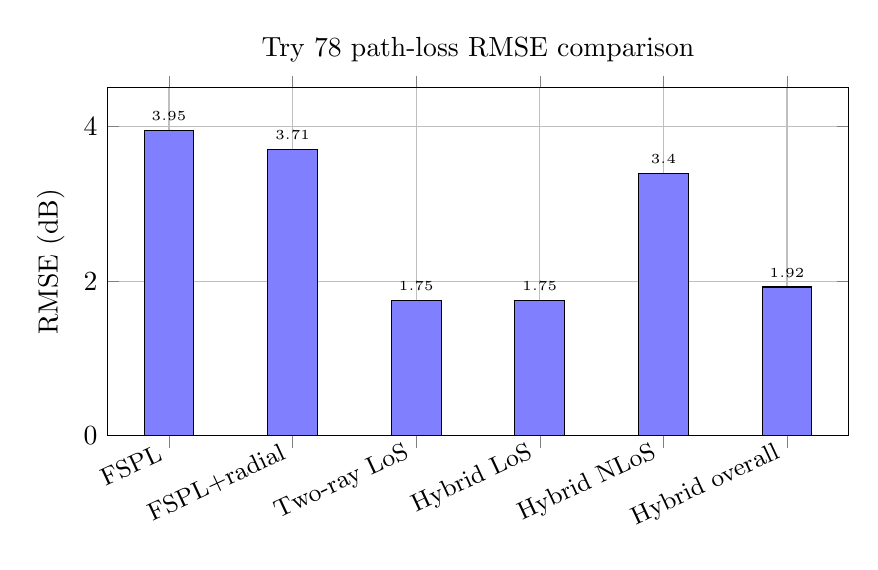
\begin{tikzpicture}
\begin{axis}[
  ybar,
  width=11cm, height=6cm,
  bar width=18pt,
  ylabel={RMSE (dB)},
  symbolic x coords={FSPL,FSPL+radial,Two-ray LoS,Hybrid LoS,Hybrid NLoS,Hybrid overall},
  xtick=data,
  x tick label style={rotate=25, anchor=east, font=\small},
  ymin=0, ymax=4.5,
  nodes near coords,
  nodes near coords align={vertical},
  every node near coord/.append style={font=\tiny},
  grid=major,
  title={Try 78 path-loss RMSE comparison}
]
\addplot[fill=blue!50] coordinates {
  (FSPL,3.9540)
  (FSPL+radial,3.7086)
  (Two-ray LoS,1.7516)
  (Hybrid LoS,1.7516)
  (Hybrid NLoS,3.3967)
  (Hybrid overall,1.9246)
};
\end{axis}
\end{tikzpicture}
\caption{Try 78 pixel-weighted RMSE values. The coherent two-ray model
reduces LoS RMSE from 3.95 dB (FSPL) to 1.75 dB, a gain of 2.2 dB.}
\label{fig:try78_rmse}
\end{figure}

\begin{figure}[H]
\centering
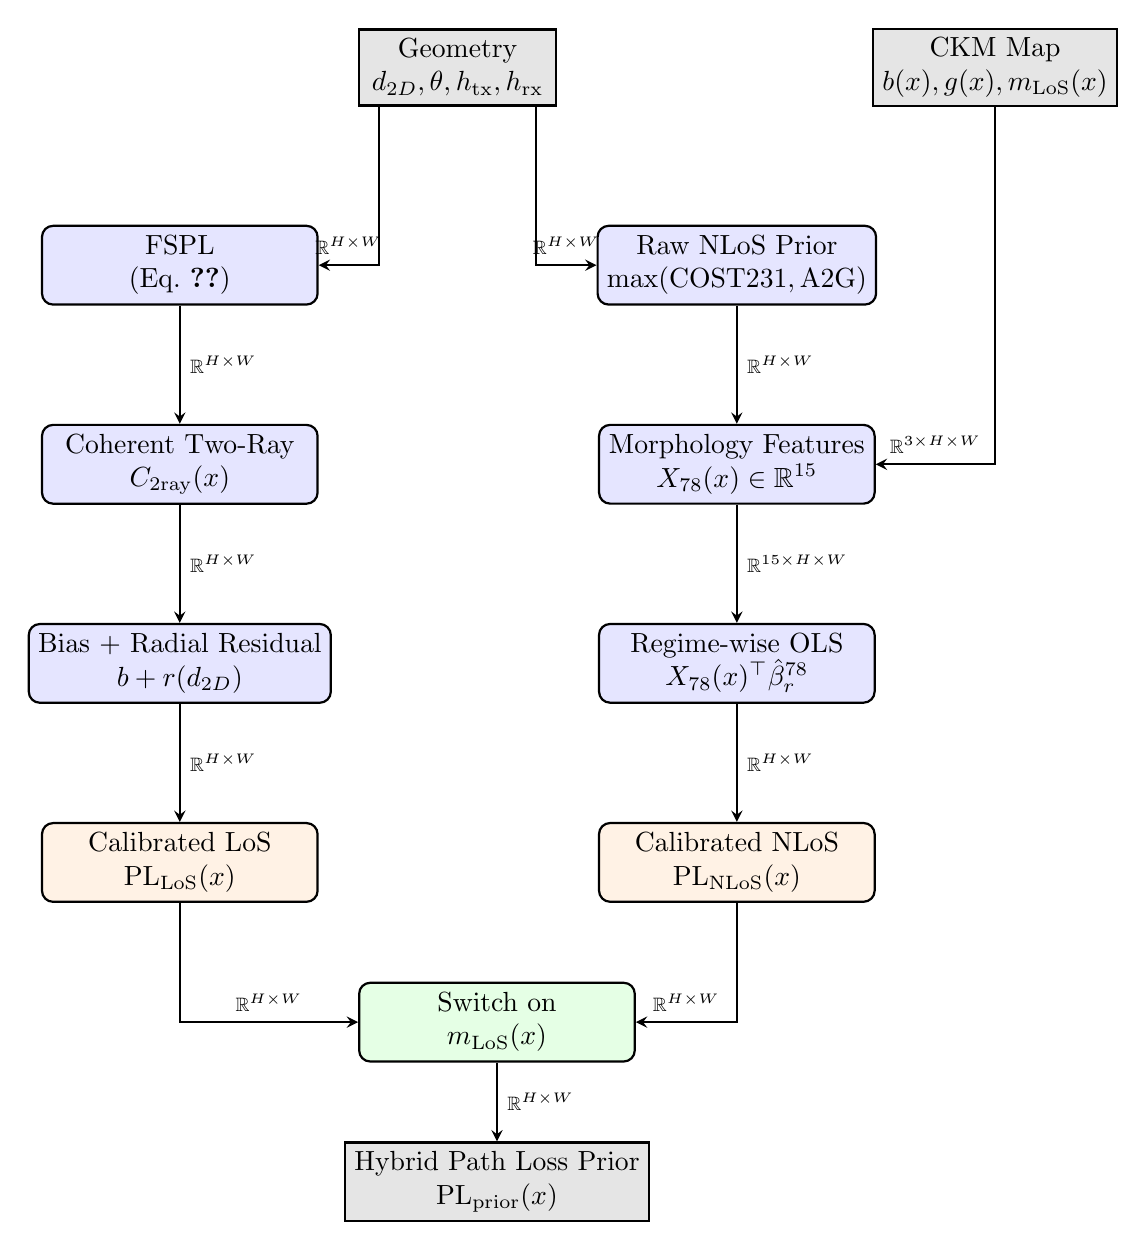
\begin{tikzpicture}[
    >=stealth,
    node distance=1cm and 2cm,
    block/.style={draw, thick, fill=blue!10, rectangle, rounded corners, minimum width=3.5cm, minimum height=1cm, align=center},
    input/.style={draw, thick, fill=gray!20, rectangle, minimum width=2.5cm, minimum height=0.8cm, align=center},
    sum/.style={draw, thick, fill=green!10, rectangle, rounded corners, minimum width=3.5cm, minimum height=1cm, align=center},
    branch/.style={draw, thick, fill=orange!10, rectangle, rounded corners, minimum width=3.5cm, minimum height=1cm, align=center}
]

% Inputs
\node[input] (geom) {Geometry \\ $d_{2D}, \theta, h_{\mathrm{tx}}, h_{\mathrm{rx}}$};
\node[input, right=4cm of geom] (map) {CKM Map \\ $b(x), g(x), m_{\mathrm{LoS}}(x)$};

% LoS Branch
\node[block, below left=1.5cm and 0.5cm of geom] (fspl) {FSPL \\ (Eq.~\ref{eq:fspl})};
\node[block, below=1.5cm of fspl] (tworay) {Coherent Two-Ray \\ $C_{\mathrm{2ray}}(x)$};
\node[block, below=1.5cm of tworay] (bias_rad) {Bias + Radial Residual \\ $b + r(d_{2D})$};
\node[branch, below=1.5cm of bias_rad] (pl_los) {Calibrated LoS \\ $\mathrm{PL}_{\mathrm{LoS}}(x)$};

\draw[->, thick] (geom.south) ++(-1,0) |- node[pos=0.75, above, font=\scriptsize] {$\mathbb{R}^{H \times W}$} (fspl.east);
\draw[->, thick] (fspl) -- node[right, font=\scriptsize] {$\mathbb{R}^{H \times W}$} (tworay);
\draw[->, thick] (tworay) -- node[right, font=\scriptsize] {$\mathbb{R}^{H \times W}$} (bias_rad);
\draw[->, thick] (bias_rad) -- node[right, font=\scriptsize] {$\mathbb{R}^{H \times W}$} (pl_los);

% NLoS Branch
\node[block, below right=1.5cm and 0.5cm of geom] (raw_nlos) {Raw NLoS Prior \\ $\max(\text{COST231}, \text{A2G})$};
\node[block, below=1.5cm of raw_nlos] (feat78) {Morphology Features \\ $X_{78}(x) \in \mathbb{R}^{15}$};
\node[block, below=1.5cm of feat78] (ols) {Regime-wise OLS \\ $X_{78}(x)^\top \hat\beta^{78}_{r}$};
\node[branch, below=1.5cm of ols] (pl_nlos) {Calibrated NLoS \\ $\mathrm{PL}_{\mathrm{NLoS}}(x)$};

\draw[->, thick] (geom.south) ++(1,0) |- node[pos=0.75, above, font=\scriptsize] {$\mathbb{R}^{H \times W}$} (raw_nlos.west);
\draw[->, thick] (map.south) |- node[pos=0.75, above, font=\scriptsize] {$\mathbb{R}^{3 \times H \times W}$} (feat78.east);
\draw[->, thick] (raw_nlos) -- node[right, font=\scriptsize] {$\mathbb{R}^{H \times W}$} (feat78);
\draw[->, thick] (feat78) -- node[right, font=\scriptsize] {$\mathbb{R}^{15 \times H \times W}$} (ols);
\draw[->, thick] (ols) -- node[right, font=\scriptsize] {$\mathbb{R}^{H \times W}$} (pl_nlos);

% Blend
\node[sum, below right=1cm and 0.5cm of pl_los] (blend) {Switch on \\ $m_{\mathrm{LoS}}(x)$};
\node[input, below=1cm of blend] (final) {Hybrid Path Loss Prior \\ $\mathrm{PL}_{\mathrm{prior}}(x)$};

\draw[->, thick] (pl_los.south) |- node[pos=0.75, above, font=\scriptsize] {$\mathbb{R}^{H \times W}$} (blend.west);
\draw[->, thick] (pl_nlos.south) |- node[pos=0.75, above, font=\scriptsize] {$\mathbb{R}^{H \times W}$} (blend.east);
\draw[->, thick] (blend) -- node[right, font=\scriptsize] {$\mathbb{R}^{H \times W}$} (final);

\end{tikzpicture}
\caption{Pipeline for the \texttt{Try 78} hybrid path loss prior. The LoS branch relies on an explicit two-ray interference model, while the NLoS branch calibrates a raw prior against map-derived morphology features using regime-wise OLS. The two branches are hard-switched based on the LoS mask to produce the final frozen prior.}
\label{fig:try78_pipeline}
\end{figure}

%% ============================================================
\section{Try 79: Delay and Angular Spread Priors}
%% ============================================================

\subsection{Physical motivation for log-domain modeling}

Delay spread (DS) and angular spread (AS) are strictly positive and
heavy-tailed statistics. Their empirical distributions are typically
log-normal, meaning $\log(1 + y)$ is approximately Gaussian
\cite{tr38901,winner2}. Modeling them in linear space would require
non-negative regression, while the log transform allows standard linear
regression tools to be applied directly.

For a spread variable $y \in \{\mathrm{DS}, \mathrm{AS}\}$, define:

\begin{equation}
z(x) = \log(1 + y(x))
\label{eq:log_transform}
\end{equation}

The $+1$ shift ensures $z \ge 0$ even when $y = 0$. The model is built to
predict $z(x)$ and then the prediction is inverted via:

\begin{equation}
\hat y(x) = \exp(\hat z(x)) - 1
\label{eq:log_invert}
\end{equation}

\subsection{Raw spread prior in log domain}

The raw log-domain prior is built as a linear combination of geometric and
morphological features:

\begin{equation}
z^{(0)}(x)
=
b_{\mathrm{LoS/NLoS}}(x)
+ b_{\mathrm{topology}}
+ a_1 \log(1+d_{2D}(x))
+ a_2 \theta_{\mathrm{inv}}(x)
+ a_3 \rho_{41}(x)
+ a_4 h_{41}(x)
+ a_5 n_{41}(x)
+ a_6 n_{41}(x)\theta_{\mathrm{inv}}(x)
\label{eq:raw_spread}
\end{equation}

where $\theta_{\mathrm{inv}}(x) = 1 - \theta_{\mathrm{norm}}(x)$ (high value
at low elevation, i.e., large off-zenith angle).

\paragraph{Interpretation of each term.}
\begin{itemize}
\item $b_{\mathrm{LoS/NLoS}}$: a baseline spread level that differs between
      LoS and NLoS. Typical values (in log-space): LoS base $\approx
      \log(1 + 4) = 1.61$ (4 ns for DS), NLoS base $\approx \log(1 + 11) =
      2.49$ (11 ns). This captures the fact that NLoS channels are richer in
      multipath and therefore exhibit larger spreads.
\item $b_{\mathrm{topology}}$: a per-topology-class additive offset, capturing
      the fact that dense high-rise urban environments typically produce larger
      spreads than open sparse environments.
\item $a_1 \log(1+d_{2D})$: distance-dependent spread growth. In 3GPP
      channel models, delay spread increases logarithmically with distance
      because farther scatterers contribute more delay \cite{tr38901}.
\item $a_2 \theta_{\mathrm{inv}}$: elevation-angle dependence. At low
      elevation angles (large $\theta_{\mathrm{inv}}$), the UAV sees more
      buildings at shallow angles, increasing both delay spread (more path
      length variation) and angular spread (wider scatterer angles).
\item $a_3 \rho_{41}$: higher building density increases spread.
\item $a_4 h_{41}$: taller buildings produce longer path length differences,
      increasing delay spread.
\item $a_5 n_{41}$: more NLoS ground pixels (more blocking) tends to increase
      spread (richer scattering environment).
\item $a_6 n_{41}\theta_{\mathrm{inv}}$: interaction: NLoS support has a
      stronger effect at low elevation angles.
\end{itemize}

Example raw prior coefficients for delay spread are:
$b_{\mathrm{LoS}} = 4.0$, $b_{\mathrm{NLoS}} = 11.0$,
$a_1 = 0.11$, $a_2 = 0.62$, $a_3 = 0.48$, $a_4 = 0.32$, $a_5 = 0.86$,
$a_6 = 0.60$.

\subsection{Calibrated spread prior}

\subsubsection{Stage 2: richer design matrix}

The raw prior $z^{(0)}(x)$ is not the final estimate. A richer 23-element
design vector is assembled:

\begin{equation}
X_{79}(x)
=
\begin{bmatrix}
z^{(0)}(x)^2 \\
z^{(0)}(x) \\
\log(1+d_{2D}(x)) \\
\theta_{\mathrm{norm}}(x) \\
\theta_{\mathrm{inv}}(x) \\
h_{\mathrm{norm}} \\
h_{\mathrm{norm}}^2 \\
\rho_{15}(x) \\
\rho_{41}(x) \\
h_{15}(x) \\
h_{41}(x) \\
n_{15}(x) \\
n_{41}(x) \\
n_{41}(x)\log(1+d_{2D}(x)) \\
\rho_{41}(x)\theta_{\mathrm{inv}}(x) \\
b_{41}(x) \\
1 \\
c_{41}(x) \\
t_{41}(x) \\
\theta_{\mathrm{norm}}(x)\rho_{41}(x) \\
c_{41}(x)\theta_{\mathrm{inv}}(x) \\
t_{41}(x)\rho_{41}(x) \\
t_{41}(x)n_{41}(x)
\end{bmatrix}
\label{eq:x79}
\end{equation}

The new features (beyond those already in $X_{78}$) are:

\paragraph{Normalized transmitter height.}

\begin{equation}
h_{\mathrm{norm}}=
\frac{\log\!\left(1+\max(h_{\mathrm{tx}}-h_{\mathrm{rx}},0)\right)}
{\log(401)}
\label{eq:hnorm}
\end{equation}

This compresses the UAV height into $[0, 1]$ on a log scale; the denominator
$\log(401)$ normalizes by the maximum expected height difference (400 m).
Both $h_{\mathrm{norm}}$ and $h_{\mathrm{norm}}^2$ are included to allow a
quadratic relationship between UAV height and spread.

\paragraph{Blocker depth.}

\begin{equation}
b_{41}(x)=
\frac{\mathrm{BoxMean}_{41}\!\left(\max(\mathrm{topology}(\cdot)-h_{\mathrm{rx}},0)\,b(\cdot)\right)(x)}
{H_{\mathrm{norm}}}
\label{eq:b41}
\end{equation}

This measures how much buildings in the $41\times 41$ window \emph{protrude}
above the receiver height. A large $b_{41}$ means there are many tall
buildings nearby, which act as diffraction edges and scatterers.

\paragraph{Transmitter clearance.}

\begin{equation}
\mathrm{clearance}(x)=\max(h_{\mathrm{tx}}-\mathrm{topology}(x),0)\,b(x)
\label{eq:clearance}
\end{equation}

\begin{equation}
c_{41}(x)=
\frac{\mathrm{BoxMean}_{41}\!\left(\mathrm{clearance}(\cdot)\right)(x)}
{H_{\mathrm{norm}}}
\label{eq:c41}
\end{equation}

This measures how far the UAV is \emph{above} surrounding buildings, i.e.,
the mean altitude clearance of the UAV over nearby building tops. A large
$c_{41}$ means the UAV is well above local rooftops, leading to better LoS
and typically smaller spread.

\paragraph{Taller-building fraction.}

\begin{equation}
t_{\mathrm{raw}}(x)=
\mathbf{1}\!\left[\mathrm{topology}(x)>h_{\mathrm{tx}}\right]\cdot b(x)
\label{eq:t_raw}
\end{equation}

\begin{equation}
t_{41}(x)=\mathrm{BoxMean}_{41}\!\left(t_{\mathrm{raw}}(\cdot)\right)(x)
\label{eq:t41}
\end{equation}

$t_{41}$ is the fraction of buildings in the $41\times 41$ window that are
taller than the UAV. A high $t_{41}$ means the UAV is operating \emph{below}
rooftop level and is more severely obstructed.

\paragraph{Interaction terms.}
Six pairwise interaction terms are included:

\begin{align}
&n_{41}(x)\log(1+d_{2D}(x)) && \text{(NLoS support vs.\ distance)}\\
&\rho_{41}(x)\theta_{\mathrm{inv}}(x) && \text{(density vs.\ elevation)}\\
&\theta_{\mathrm{norm}}(x)\rho_{41}(x) && \text{(elevation vs.\ density, complement)}\\
&c_{41}(x)\theta_{\mathrm{inv}}(x) && \text{(clearance vs.\ elevation)}\\
&t_{41}(x)\rho_{41}(x) && \text{(taller-buildings vs.\ density)}\\
&t_{41}(x)n_{41}(x) && \text{(taller-buildings vs.\ NLoS support)}
\end{align}

These allow the linear model to express, e.g., that the effect of building
density on spread depends on whether the UAV is at low or high elevation.

\subsubsection{Stage 3: regime-wise ridge regression}

The regime $r$ for Try 79 is keyed by:
\begin{itemize}
\item metric (\texttt{delay\_spread} or \texttt{angular\_spread}),
\item topology class (6 classes),
\item propagation state (LoS or NLoS),
\item antenna-height bin (low / mid / high).
\end{itemize}
This gives up to $2 \times 6 \times 2 \times 3 = 72$ regimes.

\paragraph{Calibration fitting algorithm.}
Across all training samples in regime $r$, valid pixels are selected and
subsampled at rate $p = 0.02$ (2\%). The feature matrix $\mathbf{X}_r$ and
target vector $\mathbf{z}_r = \log(1 + \mathbf{y}_r)$ (clipped to $[0, 8]$)
are accumulated. If the regime has at least $4 \times 23 = 92$ pixels, the
ridge regression is:

\begin{equation}
\hat\beta^{79}_{r}
=
\left(\mathbf{X}_r^\top \mathbf{X}_r + \lambda I_{23}\right)^{-1}
\mathbf{X}_r^\top \mathbf{z}_r,
\quad \lambda = 10^{-3}
\label{eq:ridge}
\end{equation}

The small ridge penalty $\lambda = 10^{-3}$ prevents numerical instability
when the design matrix is near-singular (e.g., when a 41$\times$41 box
feature is nearly constant across a sparse regime).

\paragraph{Normal equations.}
The normal equations for ridge regression are:

\begin{equation}
\left(\mathbf{X}_r^\top \mathbf{X}_r + \lambda I\right)
\hat\beta^{79}_{r}
=
\mathbf{X}_r^\top \mathbf{z}_r
\label{eq:normal_eqs}
\end{equation}

This is solved by Cholesky decomposition, with a fallback to
\texttt{numpy.linalg.lstsq} (minimum-norm least squares) if the matrix is
still numerically singular.

\paragraph{Accumulation trick for large datasets.}
Since the CKM dataset contains $\sim$10\,840 training samples and each sample
contributes $O(10^4)$ pixels, forming the full $\mathbf{X}_r$ matrix in
memory would be prohibitive. Instead, the sufficient statistics
$\mathbf{X}_r^\top\mathbf{X}_r$ ($23\times 23$) and $\mathbf{X}_r^\top
\mathbf{z}_r$ ($23\times 1$) are accumulated incrementally:

\begin{align}
\mathbf{A}_r &\mathrel{+}= \mathbf{X}_{r,s}^\top \mathbf{X}_{r,s} \quad \forall s\\
\mathbf{v}_r &\mathrel{+}= \mathbf{X}_{r,s}^\top \mathbf{z}_{r,s} \quad \forall s
\end{align}

where $s$ indexes training samples, and only $\mathbf{A}_r$ and $\mathbf{v}_r$
need to be stored. The ridge solution is then $\hat\beta^{79}_{r} = (\mathbf{A}_r
+ \lambda I)^{-1} \mathbf{v}_r$.

\paragraph{Fallback hierarchy.}
If a regime is too sparse to fit ($< 92$ pixels), the code falls back to
progressively more general regimes:

\begin{enumerate}
\item exact regime: (metric, topology class, LoS/NLoS, antenna bin),
\item same topology class + LoS/NLoS + \emph{all} antenna heights,
\item same topology class + \emph{all} LoS states + all antenna heights,
\item global topology + LoS/NLoS + all antenna heights,
\item fully global fallback: (metric, global, all-LoS, all-ant).
\end{enumerate}

This ensures that even data-sparse regimes always have a valid coefficient
vector, at the cost of lower specificity.

\paragraph{Example fitted coefficients.}
For the regime \texttt{delay\_spread|open\_sparse\_vertical|LoS|mid\_ant}:
\[
\hat\beta^{79} =
\begin{bmatrix}
-1.020,\ 9.974,\ -1.030,\ -4.530,\ -6.412,\ 11.724,\ -9.017,\ -0.973,\
-1.849,\ -2.806,\ -1.578,\ -1.110 \\[4pt]
-6.950,\ 0.540,\ 0.521,\ 6.621,\ -10.929,\ 0.267,\ 3.567,\ -2.367,\
1.058,\ -15.276,\ -3.614
\end{bmatrix}^\top
\]
The large positive weight on $z^{(0)}$ ($\beta_2 = 9.97$) and negative bias
($\beta_{17} = -10.93$) together calibrate the scale of the raw prior.

\subsubsection{Stage 4: inverse transform and clipping}

Once the calibrated log-domain prediction $\hat z(x) = X_{79}(x)^\top
\hat\beta^{79}_{r}$ is obtained, it is mapped back to native units:

\begin{equation}
\hat y(x)
=
\exp\left(\hat z(x)\right)-1
\label{eq:inv_log}
\end{equation}

Then regime-dependent clipping is applied:

\begin{equation}
\hat y(x)
=
\begin{cases}
\mathrm{clip}\left(\hat y(x),0,y_{\max}^{\mathrm{LoS}}\right), & m_{\mathrm{LoS}}(x)=1 \\
\mathrm{clip}\left(\hat y(x),0,y_{\max}^{\mathrm{NLoS}}\right), & m_{\mathrm{LoS}}(x)=0
\end{cases}
\label{eq:spread_clip}
\end{equation}

The clip limits are:
\begin{itemize}
\item delay spread: $y_{\max}^{\mathrm{LoS}} = y_{\max}^{\mathrm{NLoS}} = 400$ ns,
\item angular spread: $y_{\max}^{\mathrm{LoS}} = 15^\circ$,
      $y_{\max}^{\mathrm{NLoS}} = 90^\circ$.
\end{itemize}

The LoS angular spread clip of $15^\circ$ reflects that in LoS conditions the
direct ray dominates and the angular energy is concentrated near the direction
of the UAV; in NLoS, the full $90^\circ$ hemisphere is accessible via
diffraction and scattering.

\begin{figure}[H]
\centering
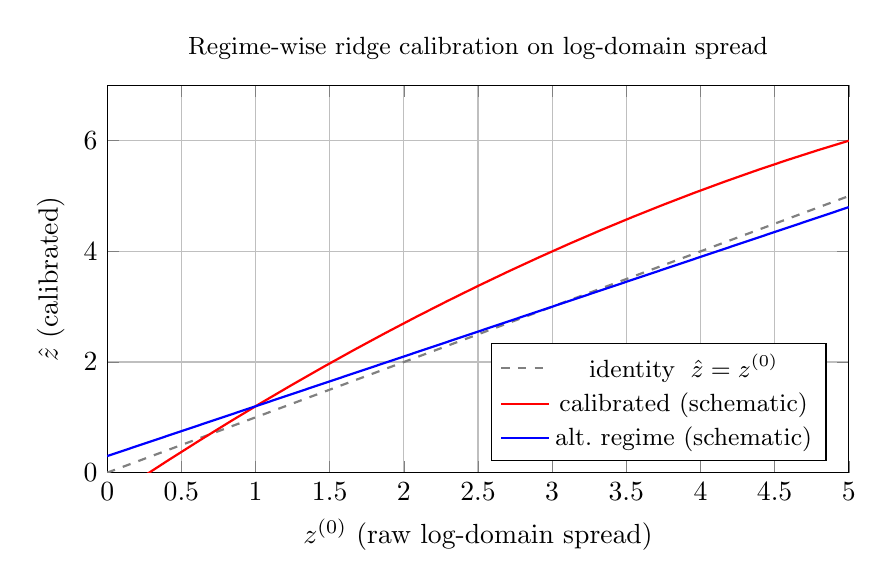
\begin{tikzpicture}
\begin{axis}[
  width=11cm, height=6.5cm,
  xlabel={$z^{(0)}$ (raw log-domain spread)},
  ylabel={$\hat{z}$ (calibrated)},
  xmin=0, xmax=5,
  ymin=0, ymax=7,
  grid=major,
  legend style={
    at={(0.97,0.03)},
    anchor=south east,
    font=\small,
    cells={align=left}
  },
  title style={font=\small},
  title={Regime-wise ridge calibration on log-domain spread}
]
\addplot[thick, gray, dashed, domain=0:5] {x};
\addlegendentry{identity\; $\hat{z} = z^{(0)}$}
\addplot[thick, red, domain=0:5] {-0.5 + 1.8*x - 0.1*x^2};
\addlegendentry{calibrated (schematic)}
\addplot[thick, blue, domain=0:5] {0.3 + 0.9*x};
\addlegendentry{alt.\ regime (schematic)}
\end{axis}
\end{tikzpicture}
\caption{Schematic illustration of the regime-wise calibration. The raw
log-domain prior $z^{(0)}$ (identity line) is mapped by the fitted linear
model to the calibrated prediction $\hat{z}$. Different regimes produce
different calibration curves, allowing the model to correct for systematic
biases in the raw prior on a per-scene basis.}
\label{fig:spread_cal}
\end{figure}

\subsection{Observed Try 79 results}

All values follow the pixel-weighted RMSE definition of
Section~\ref{sec:pw_metric}: metrics are pooled across all valid \emph{ground}
pixels, buildings excluded, and a single square root is taken over the
accumulated SSE.

\subsubsection{Delay spread}

\begin{table}[H]
\centering
\caption{Delay spread: calibrated test RMSE (ns) by topology class.}
\label{tab:ds_topo}
\begin{tabular}{lccc}
\toprule
Topology class & Overall & LoS & NLoS \\
\midrule
open\_sparse\_lowrise      & 16.8807 & 17.0146 & 15.4284 \\
open\_sparse\_vertical     & 40.8366 & 40.4400 & 44.0772 \\
mixed\_compact\_lowrise    & 17.2661 & 16.6524 & 18.9097 \\
mixed\_compact\_midrise    & 37.8812 & 38.2608 & 37.2474 \\
dense\_block\_midrise      & 26.9047 & 28.9951 & 25.0188 \\
dense\_block\_highrise     & 43.5159 & 40.1619 & 45.0775 \\
\midrule
\textbf{Overall}           & \textbf{28.1023} & \textbf{27.4851} & \textbf{29.6157} \\
\bottomrule
\end{tabular}
\end{table}

\begin{table}[H]
\centering
\caption{Delay spread: calibrated test RMSE (ns) by antenna-height bin.}
\label{tab:ds_ant}
\begin{tabular}{lccc}
\toprule
Antenna bin & Overall & LoS & NLoS \\
\midrule
low\_ant  & 37.3435 & 39.7087 & 33.5247 \\
mid\_ant  & 29.0487 & 28.4214 & 30.5248 \\
high\_ant & 12.2353 & 12.1513 & 12.6785 \\
\bottomrule
\end{tabular}
\end{table}

\subsubsection{Angular spread}

\begin{table}[H]
\centering
\caption{Angular spread: calibrated test RMSE ($^\circ$) by topology class.}
\label{tab:as_topo}
\begin{tabular}{lccc}
\toprule
Topology class & Overall & LoS & NLoS \\
\midrule
open\_sparse\_lowrise      & 10.0141 & 10.3006 & 6.3311 \\
open\_sparse\_vertical     & 12.6999 & 12.9825 & 9.9658 \\
mixed\_compact\_lowrise    & 14.3745 & 15.9870 & 8.1715 \\
mixed\_compact\_midrise    & 15.2580 & 17.8463 & 9.5741 \\
dense\_block\_midrise      & 15.5326 & 21.2010 & 8.1714 \\
dense\_block\_highrise     & 14.6372 & 21.3260 & 9.7809 \\
\midrule
\textbf{Overall}           & \textbf{13.7416} & \textbf{15.2818} & \textbf{8.6614} \\
\bottomrule
\end{tabular}
\end{table}

\begin{table}[H]
\centering
\caption{Angular spread: calibrated test RMSE ($^\circ$) by antenna-height bin.}
\label{tab:as_ant}
\begin{tabular}{lccc}
\toprule
Antenna bin & Overall & LoS & NLoS \\
\midrule
low\_ant  & 15.5124 & 18.4271 & 9.6818 \\
mid\_ant  & 14.4554 & 16.2652 & 8.5643 \\
high\_ant & 10.8852 & 11.6030 & 5.6148 \\
\bottomrule
\end{tabular}
\end{table}

\begin{figure}[H]
\centering
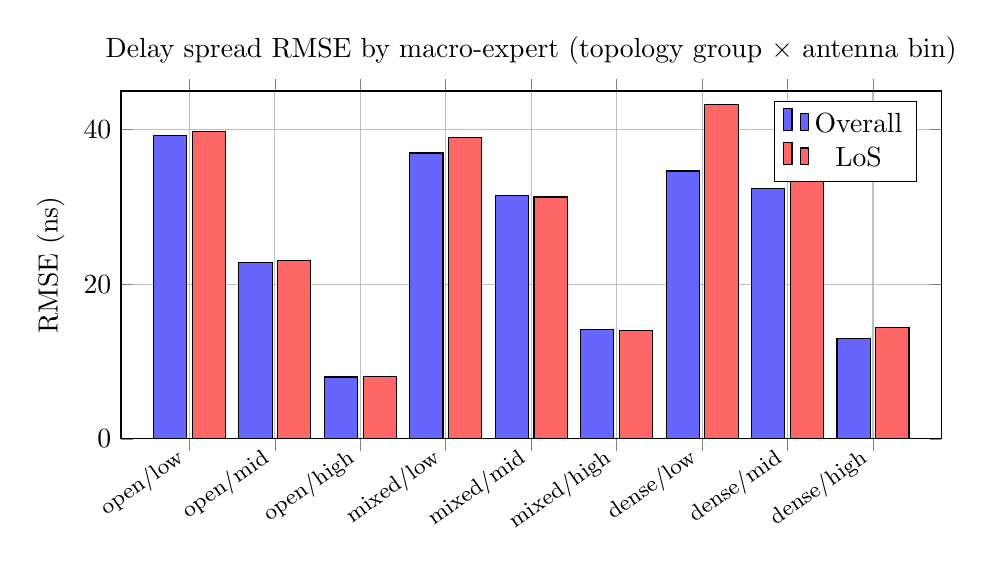
\begin{tikzpicture}
\begin{axis}[
  ybar, bar width=12pt,
  width=12cm, height=6cm,
  ylabel={RMSE (ns)},
  symbolic x coords={
    open/low, open/mid, open/high,
    mixed/low, mixed/mid, mixed/high,
    dense/low, dense/mid, dense/high
  },
  xtick=data,
  x tick label style={rotate=35, anchor=east, font=\footnotesize},
  ymin=0, ymax=45,
  grid=major,
  legend pos=north east,
  title={Delay spread RMSE by macro-expert (topology group $\times$ antenna bin)}
]
\addplot[fill=blue!60] coordinates {
  (open/low,39.2361)(open/mid,22.8110)(open/high,7.9965)
  (mixed/low,36.9733)(mixed/mid,31.4652)(mixed/high,14.1209)
  (dense/low,34.6513)(dense/mid,32.3963)(dense/high,13.0220)
};
\addlegendentry{Overall}
\addplot[fill=red!60] coordinates {
  (open/low,39.6989)(open/mid,23.0193)(open/high,8.0807)
  (mixed/low,39.0233)(mixed/mid,31.2783)(mixed/high,13.9754)
  (dense/low,43.2713)(dense/mid,34.3216)(dense/high,14.4157)
};
\addlegendentry{LoS}
\end{axis}
\end{tikzpicture}
\caption{Delay spread RMSE (ns) broken down by topology macro-group and
antenna-height bin. High-altitude UAVs (high\_ant) consistently achieve the
lowest RMSE across all topology groups.}
\label{fig:ds_macroexpert}
\end{figure}

\begin{figure}[H]
\centering
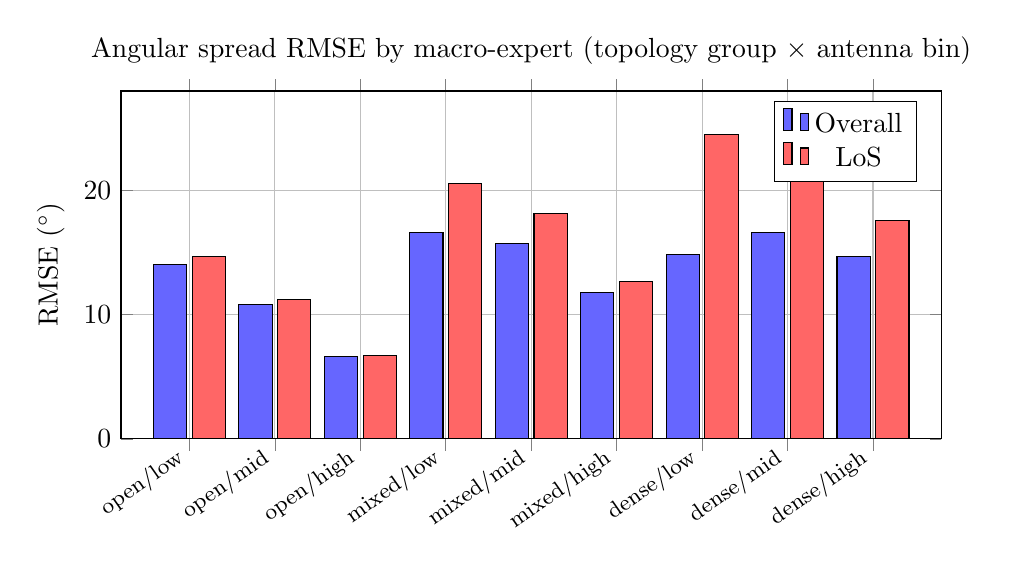
\begin{tikzpicture}
\begin{axis}[
  ybar, bar width=12pt,
  width=12cm, height=6cm,
  ylabel={RMSE ($^\circ$)},
  symbolic x coords={
    open/low, open/mid, open/high,
    mixed/low, mixed/mid, mixed/high,
    dense/low, dense/mid, dense/high
  },
  xtick=data,
  x tick label style={rotate=35, anchor=east, font=\footnotesize},
  ymin=0, ymax=28,
  grid=major,
  legend pos=north east,
  title={Angular spread RMSE by macro-expert (topology group $\times$ antenna bin)}
]
\addplot[fill=blue!60] coordinates {
  (open/low,14.0519)(open/mid,10.8252)(open/high,6.6304)
  (mixed/low,16.6418)(mixed/mid,15.7295)(mixed/high,11.7761)
  (dense/low,14.8324)(dense/mid,16.5990)(dense/high,14.6778)
};
\addlegendentry{Overall}
\addplot[fill=red!60] coordinates {
  (open/low,14.6689)(open/mid,11.2022)(open/high,6.7387)
  (mixed/low,20.5825)(mixed/mid,18.1483)(mixed/high,12.6994)
  (dense/low,24.4895)(dense/mid,23.2247)(dense/high,17.5535)
};
\addlegendentry{LoS}
\end{axis}
\end{tikzpicture}
\caption{Angular spread RMSE ($^\circ$) broken down by topology macro-group
and antenna-height bin. The LoS RMSE is notably higher than NLoS RMSE in
dense scenarios because LoS angular spread is dominated by a direct ray
spike, which is harder to localize precisely.}
\label{fig:as_macroexpert}
\end{figure}

\begin{figure}[H]
\centering
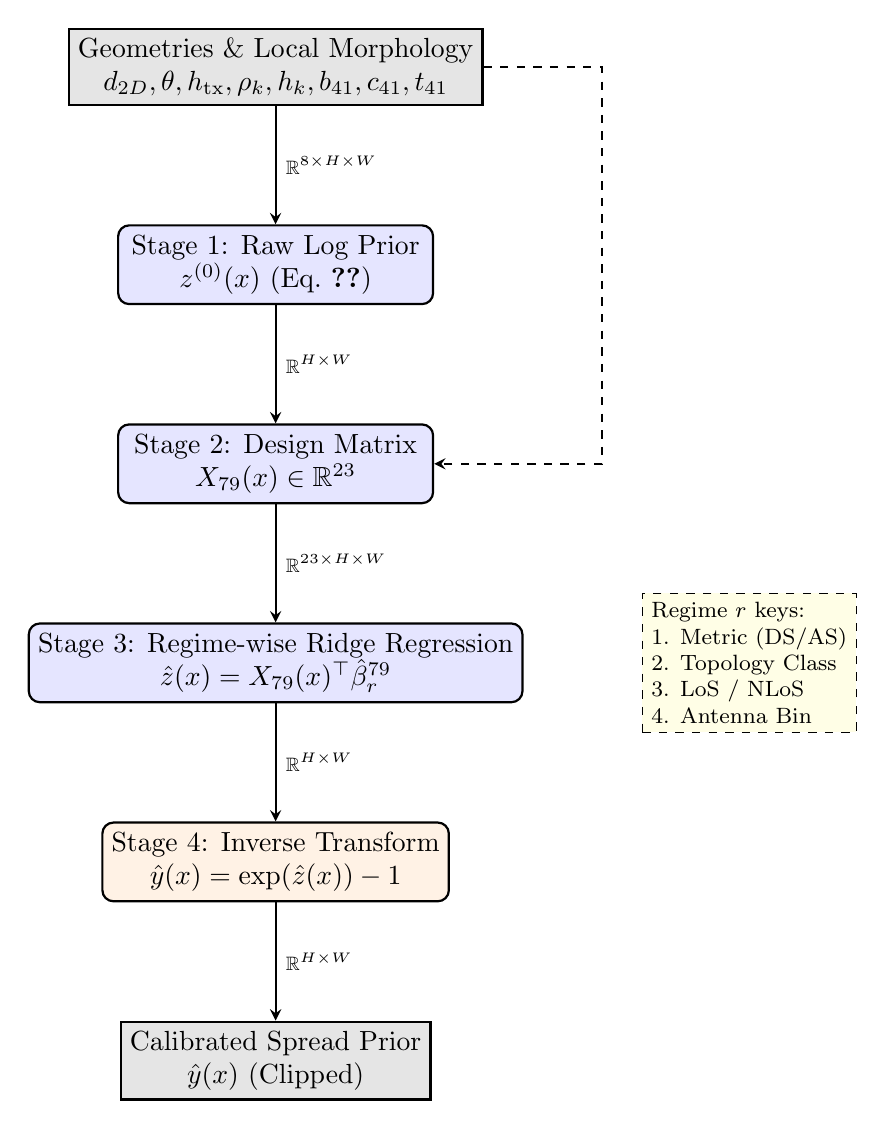
\begin{tikzpicture}[
    >=stealth,
    node distance=1.5cm and 2cm,
    block/.style={draw, thick, fill=blue!10, rectangle, rounded corners, minimum width=4cm, minimum height=1cm, align=center},
    input/.style={draw, thick, fill=gray!20, rectangle, minimum width=2.5cm, minimum height=0.8cm, align=center},
    sum/.style={draw, thick, fill=green!10, circle, minimum size=0.8cm, align=center},
    branch/.style={draw, thick, fill=orange!10, rectangle, rounded corners, minimum width=3cm, minimum height=1cm, align=center}
]

% Inputs
\node[input] (inputs) {Geometries \& Local Morphology \\ $d_{2D}, \theta, h_{\mathrm{tx}}, \rho_k, h_k, b_{41}, c_{41}, t_{41}$};

% Pipeline
\node[block, below=1.5cm of inputs] (raw_prior) {Stage 1: Raw Log Prior \\ $z^{(0)}(x)$ (Eq.~\ref{eq:raw_spread})};
\node[block, below=1.5cm of raw_prior] (features) {Stage 2: Design Matrix \\ $X_{79}(x) \in \mathbb{R}^{23}$};
\node[block, below=1.5cm of features] (ridge) {Stage 3: Regime-wise Ridge Regression \\ $\hat z(x) = X_{79}(x)^\top \hat\beta^{79}_{r}$};
\node[branch, below=1.5cm of ridge] (invert) {Stage 4: Inverse Transform \\ $\hat y(x) = \exp(\hat z(x)) - 1$};
\node[input, below=1.5cm of invert] (clip) {Calibrated Spread Prior \\ $\hat y(x)$ (Clipped)};

% Connections
\draw[->, thick] (inputs) -- node[right, font=\scriptsize] {$\mathbb{R}^{8 \times H \times W}$} (raw_prior);
\draw[->, thick] (raw_prior) -- node[right, font=\scriptsize] {$\mathbb{R}^{H \times W}$} (features);
\draw[->, thick] (features) -- node[right, font=\scriptsize] {$\mathbb{R}^{23 \times H \times W}$} (ridge);
\draw[->, thick] (ridge) -- node[right, font=\scriptsize] {$\mathbb{R}^{H \times W}$} (invert);
\draw[->, thick] (invert) -- node[right, font=\scriptsize] {$\mathbb{R}^{H \times W}$} (clip);

% Bypass from inputs to features
\draw[->, thick, dashed] (inputs.east) -| ++(1.5,-1.5) |- (features.east);

% Regime conditions
\node[draw, dashed, fill=yellow!10, right=1.5cm of ridge, align=left, font=\footnotesize] {Regime $r$ keys:\\1. Metric (DS/AS)\\2. Topology Class\\3. LoS / NLoS\\4. Antenna Bin};

\end{tikzpicture}
\caption{Pipeline for the \texttt{Try 79} delay and angular spread priors. Both spread modalities share this identical linear architecture. They predict the expected spread in the log domain using regime-wise ridge regression over 23 spatial and geometric features.}
\label{fig:try79_pipeline}
\end{figure}

%% ============================================================
\section{What is reused in Try 80, and what is new}
%% ============================================================

\subsection{What is not new in Try 80}

The following are inherited and frozen:

\begin{itemize}
\item the calibrated two-ray LoS path-loss prior from \texttt{Try 78}
      (Eq.~\ref{eq:pl_los}),
\item the calibrated regime-wise NLoS path-loss prior from \texttt{Try 78}
      (Eq.~\ref{eq:pl_nlos_final}),
\item the calibrated delay-spread prior from \texttt{Try 79}
      (Eq.~\ref{eq:inv_log}),
\item the calibrated angular-spread prior from \texttt{Try 79}
      (Eq.~\ref{eq:inv_log}).
\end{itemize}

\subsection{Experimental protocol and reporting status}

\texttt{Try 80} follows the same strict split philosophy as the recent
distribution-first tries. The split is a city-holdout split with
\texttt{split\_seed = 42}, \texttt{val\_ratio = 0.15}, and
\texttt{test\_ratio = 0.15}. Metrics and losses are computed only on valid
ground pixels, using the target-specific no-data masks and the explicit
LoS/NLoS masks. The model input contains nine spatial channels:

\begin{enumerate}
\item normalized topology,
\item LoS mask,
\item NLoS mask,
\item ground mask,
\item combined path-loss prior,
\item LoS path-loss prior,
\item NLoS path-loss prior,
\item delay-spread prior,
\item angular-spread prior.
\end{enumerate}

The scalar UAV height is not appended as a constant image channel. It is
encoded with a sinusoidal embedding and injected into the network through FiLM
conditioning. The default \texttt{try80\_joint\_big} configuration uses a
shared encoder-decoder with \texttt{base\_width = 96}, three GMM components
per task and region, \(\alpha\)-gate bias \(-2\), and fixed residual caps
specified separately for path loss, delay spread and angular spread.

Because the full \texttt{Try 80} run is still in training, this note does not
claim final numerical improvements for the deep model. Final validation/test
tables should be inserted only after the selected checkpoint and test
evaluation are frozen. Until then, the quantitative tables in this document
should be interpreted as documenting the frozen \texttt{Try 78}/\texttt{Try 79}
priors and the calibration assets consumed by \texttt{Try 80}, not as final
\texttt{Try 80} performance claims.

\subsection{What is new in Try 80}

\texttt{Try 80} introduces a joint multi-task architecture that predicts a
\emph{Gaussian Mixture Model (GMM)} at each pixel, rather than a simple point
estimate. For each task $k \in \{\mathrm{PL},\, \mathrm{DS},\, \mathrm{AS}\}$,
the target value $y_k(x)$ is modeled as being drawn from a mixture of $J=3$ components.

The mean of each mixture component $j$ is anchored to the frozen prior:

\begin{equation}
\mu_{k,j}(x)
=
y^{\mathrm{prior}}_k(x)
+
\alpha_k(x) \cdot
\mathrm{clip}\left(
\delta_{\mathrm{global},k,j} + \delta_{\mathrm{local},k}(x),
\pm\delta_{\max,k}
\right)
\label{eq:try80_mu}
\end{equation}

where:
\begin{itemize}
\item $y^{\mathrm{prior}}_k(x)$ is the frozen prior from \texttt{Try 78}
      or \texttt{Try 79},
\item $\delta_{\mathrm{global},k,j}$ is a map-level residual offset for component $j$,
\item $\delta_{\mathrm{local},k}(x)$ is a per-pixel residual refinement shared across components,
\item $\alpha_k(x) \in (0,1)$ is a learned spatial gating factor,
\item The sum is bounded to $\pm\delta_{\max,k}$ to prevent the DNN from
      deviating catastrophically from the prior.
\end{itemize}

The DNN also predicts the per-pixel mixture probabilities $p_{k,j}(x)$ and
component variances $\sigma_{k,j}^2(x) = \sigma_{\mathrm{global},k,j}^2 +
\tilde\sigma_{\mathrm{local},k}^2(x)$.

The model is trained end-to-end to maximize the Negative Log Likelihood (NLL)
of the measurements under this GMM. The deterministic point prediction used for
RMSE evaluation is the expected value of the mixture:

\begin{equation}
\hat y_k(x) = \sum_{j=1}^3 p_{k,j}(x) \mu_{k,j}(x)
\label{eq:try80_point}
\end{equation}

The training loss also includes a prior-preservation term:

\begin{equation}
\mathcal{L}
=
\mathcal{L}_{\mathrm{task}}
+ \lambda_{\mathrm{prior}}
\sum_{k}
\mathbb{E}_{x}\!\left[\max\left(0,\,
\left(\hat y_k(x) - y_k(x)\right)^2 - \left(y^{\mathrm{prior}}_k(x) - y_k(x)\right)^2
\right)\right]
\label{eq:try80_loss}
\end{equation}

The second term is a \emph{pixel-wise} prior-guard. It penalizes the model
explicitly on any pixel where its squared error exceeds the prior's squared
error. This asymmetric penalty is strictly stronger than an aggregate RMSE
check, as it prevents the DNN from sacrificing performance in difficult local
regions to optimize the global mean.

The four components of the Try 80 pipeline are therefore:

\begin{enumerate}
\item inject frozen priors as explicit map-shaped input channels,
\item multi-task DNN predicts a per-pixel GMM anchored to the prior,
\item train via NLL alongside a pixel-wise prior-preserving loss term,
\item final point prediction is the expected value of the mixture.
\end{enumerate}

\subsection{Novelty relative to common implementations}

Compared with common deep-learning implementations for radio-map prediction,
\texttt{Try 80} differs in several practical ways:

\begin{enumerate}
\item \textbf{It is not a black-box image-to-image regressor.}
      A common approach is to feed the topology map, transmitter position and
      height to a UNet-like model and let the network learn the full target
      map directly. \texttt{Try 80} instead gives the network calibrated
      physics/statistics priors and asks it to learn only the residual part.

\item \textbf{The residual is bounded in native physical units.}
      The network cannot move arbitrarily far from the prior. The residual caps
      are specified in dB for path loss, ns for delay spread, and degrees for
      angular spread. This is more constrained than ordinary residual learning,
      where the residual branch is typically unconstrained.

\item \textbf{The prior is protected pixel by pixel, not only on average.}
      Many hybrid models compare against a baseline only through aggregate RMSE.
      Here, the prior guard penalizes individual pixels where the learned model
      becomes worse than the frozen prior, discouraging the model from trading
      local degradation for a small global improvement.

\item \textbf{LoS and NLoS are explicit regions inside the head.}
      Instead of expecting one shared output distribution to cover both regimes,
      the model predicts separate LoS and NLoS mixture structures and then
      selects the appropriate regional prediction using the geometry mask.

\item \textbf{Global scenario uncertainty and local spatial corrections are
      separated.}
      The global head predicts map-level mixture structure from pooled context,
      while the local head predicts per-pixel residual refinements. This is
      different from a standard fully convolutional head, where global and
      local effects are mixed implicitly in the same output tensor.

\item \textbf{The same architecture couples three related propagation targets.}
      Instead of training independent models for path loss, delay spread and
      angular spread, \texttt{Try 80} shares the spatial representation and
      height conditioning while keeping task-specific probabilistic heads.

\item \textbf{Uncertainty is modeled around a prior, not around zero.}
      The GMM components describe plausible residual modes relative to the
      calibrated physical/statistical prediction. This is different from a
      conventional mixture-density network that directly models the absolute
      target distribution.

\item \textbf{The model remains inspectable after training.}
      The residual gates, capped offsets, global mixture weights, LoS/NLoS
      branches and frozen prior maps can be inspected separately. This makes
      failure analysis easier than in a single unconstrained dense output map.
\end{enumerate}

\subsubsection{Architecture: Shared UNet with FiLM}

Under the hood, \texttt{Try 80} processes the map inputs (such as building layouts and LoS/NLoS masks) through a shared multi-task convolutional encoder-decoder. Because the UAV altitude strongly modifies propagation paths, it is insufficient to simply append the scalar UAV height to the spatial input. Instead, the scalar UAV height is encoded into a condition vector $\mathbf{c} \in \mathbb{R}^{128}$ and injected dynamically into the convolutional feature maps at multiple scales via \emph{Feature-wise Linear Modulation (FiLM)} layers. 

For a given convolutional feature map $\mathbf{X} \in \mathbb{R}^{C \times H \times W}$, a linear projection of the height condition $\mathbf{c}$ outputs a scale vector $\boldsymbol{\gamma} \in \mathbb{R}^C$ and a shift vector $\boldsymbol{\beta} \in \mathbb{R}^C$. The feature map is then modulated via an affine transformation:
\begin{equation}
\mathbf{X}' = \mathbf{X} \odot (1 + \boldsymbol{\gamma}) + \boldsymbol{\beta}
\label{eq:film}
\end{equation}
where $\boldsymbol{\gamma}$ and $\boldsymbol{\beta}$ are broadcasted spatially across the height and width. This mechanism allows the scalar altitude to globally scale and shift the activation of specific spatial filters—for instance, amplifying ''far-field scattering'' filters at high altitudes while suppressing them at low altitudes.

The architecture explicitly enforces the separation of global and local effects via a dual-head design for each task, directly mirroring the mathematical separation of $(x)$-dependent and non-$(x)$-dependent variables in Eq.~\ref{eq:try80_mu}:

\begin{itemize}
\item \textbf{Global Head (Map-Level Context)}: The deepest bottleneck feature map is globally average-pooled over its spatial dimensions to produce a single vector representing the macro-context of the entire map (e.g., ''this is predominantly a dense high-rise environment''). This pooled vector, fused with the height condition, is passed through a Multi-Layer Perceptron (MLP) to predict the non-spatial quantities: mixture probabilities $p_{k,j}$, global offsets $\delta_{\mathrm{global},k,j}$, and global variances $\sigma_{\mathrm{global},k,j}^2$. These apply equally to all pixels, capturing the base scenario behavior.

\item \textbf{Local Head (Pixel-Level Refinement)}: The high-resolution output of the decoder ($\mathbf{F} \in \mathbb{R}^{C' \times H \times W}$) is passed through $1\times1$ convolutions to predict the spatially varying fields. It outputs 1-channel maps for the residual refinement $\delta_{\mathrm{local},k}(x)$, the spatial gating factor $\alpha_k(x)$, and the local variance $\tilde\sigma_{\mathrm{local},k}^2(x)$. Because these terms are derived from the high-resolution spatial decoder branch, they react to micro-morphological corrections, like the specific placement of a building blocking the path.
\end{itemize}

This guarantees that broad contextual shifts (e.g., an entire map having systematically higher delay spread) are modeled separately from fine-grained morphological effects (e.g., a specific street canyon creating a localized multipath trap).

\begin{figure}[H]
\centering
\resizebox{\textwidth}{!}{%
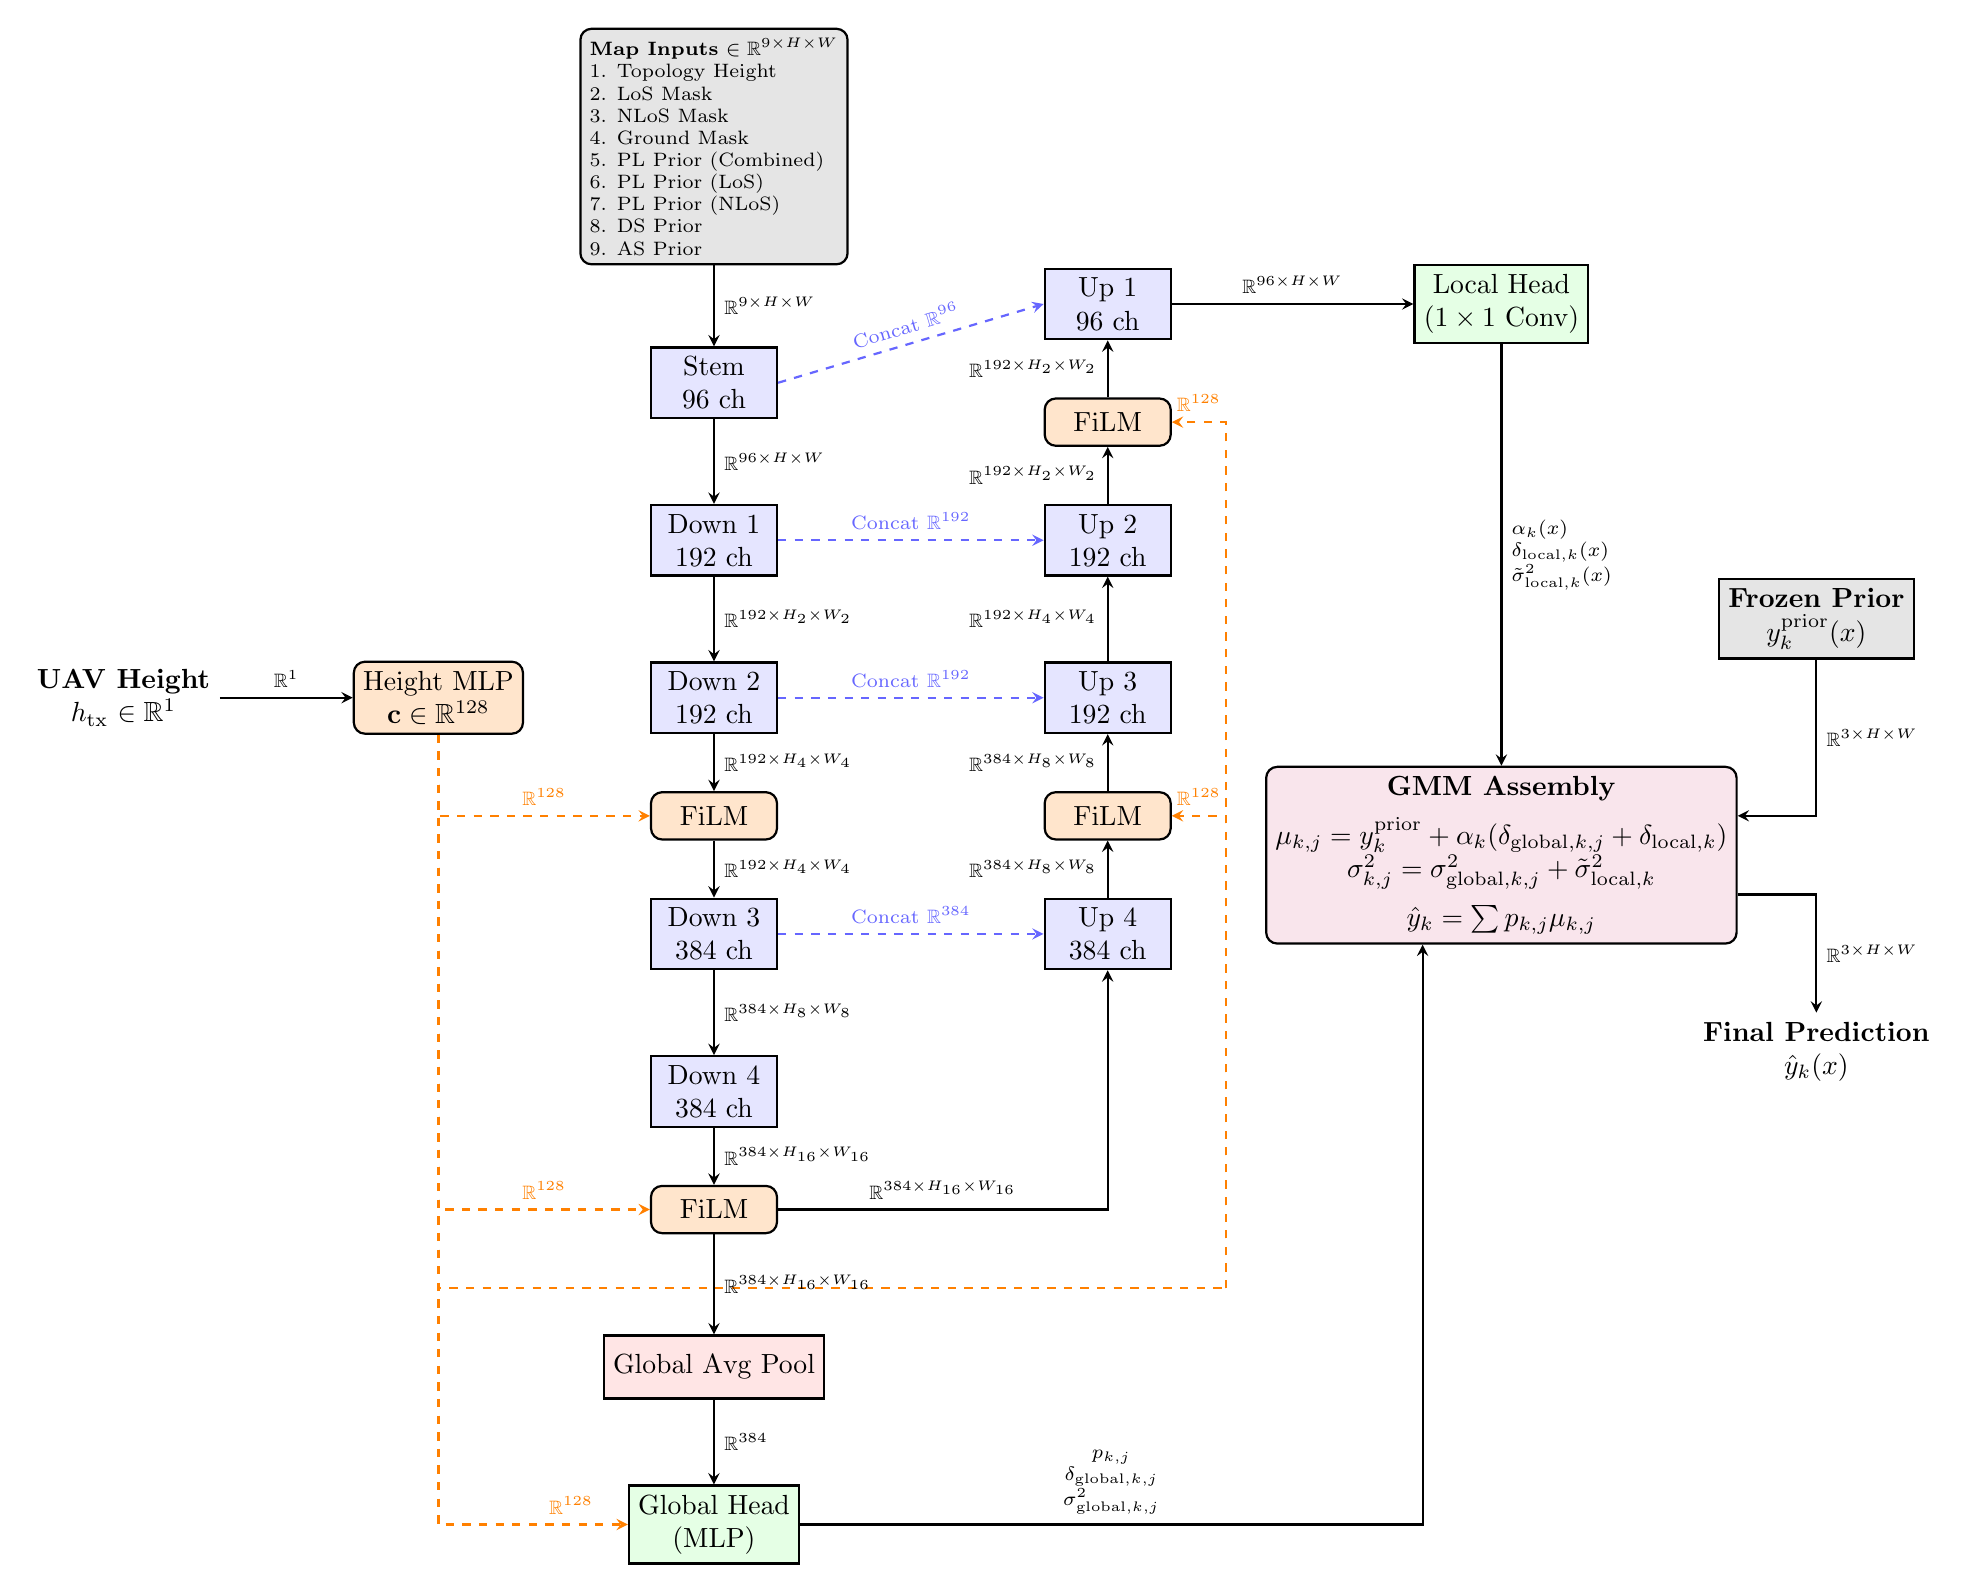
\begin{tikzpicture}[
    >=stealth,
    block/.style={draw, thick, fill=blue!10, rectangle, minimum width=1.6cm, minimum height=0.8cm, align=center},
    pool/.style={draw, thick, fill=red!10, rectangle, minimum width=1.6cm, minimum height=0.8cm, align=center},
    film/.style={draw, thick, fill=orange!20, rectangle, rounded corners, minimum width=1.6cm, minimum height=0.6cm, align=center},
    head/.style={draw, thick, fill=green!10, rectangle, minimum width=2cm, minimum height=0.8cm, align=center},
    gmm/.style={draw, thick, fill=purple!10, rectangle, rounded corners, minimum width=3.5cm, minimum height=2cm, align=center},
    skip/.style={->, thick, blue!60, dashed}
]

% Inputs
\node[align=left, font=\scriptsize, draw, thick, fill=gray!20, rectangle, rounded corners] (in_map) at (0, 3) {\textbf{Map Inputs} $\in \mathbb{R}^{9 \times H \times W}$ \\ 1. Topology Height \\ 2. LoS Mask \\ 3. NLoS Mask \\ 4. Ground Mask \\ 5. PL Prior (Combined) \\ 6. PL Prior (LoS) \\ 7. PL Prior (NLoS) \\ 8. DS Prior \\ 9. AS Prior};
\node[align=center] (in_htx) at (-7.5, -4) {\textbf{UAV Height} \\ $h_{\mathrm{tx}}$ $\in \mathbb{R}^{1}$};

% Height MLP
\node[film] (h_mlp) at (-3.5, -4) {Height MLP \\ $\mathbf{c} \in \mathbb{R}^{128}$};
\draw[->, thick] (in_htx) -- node[above, font=\scriptsize] {$\mathbb{R}^{1}$} (h_mlp);

% Encoder (Left Column)
\node[block] (e0) at (0, 0) {Stem \\ 96 ch};
\node[block] (e1) at (0, -2) {Down 1 \\ 192 ch};
\node[block] (e2) at (0, -4) {Down 2 \\ 192 ch};
\node[film] (f2) at (0, -5.5) {FiLM};
\node[block] (e3) at (0, -7) {Down 3 \\ 384 ch};
\node[block] (e4) at (0, -9) {Down 4 \\ 384 ch};
\node[film] (f4) at (0, -10.5) {FiLM};

\draw[->, thick] (in_map) -- node[right, font=\scriptsize] {$\mathbb{R}^{9 \times H \times W}$} (e0);
\draw[->, thick] (e0) -- node[right, font=\scriptsize] {$\mathbb{R}^{96 \times H \times W}$} (e1);
\draw[->, thick] (e1) -- node[right, font=\scriptsize] {$\mathbb{R}^{192 \times H_2 \times W_2}$} (e2);
\draw[->, thick] (e2) -- node[right, font=\scriptsize] {$\mathbb{R}^{192 \times H_4 \times W_4}$} (f2);
\draw[->, thick] (f2) -- node[right, font=\scriptsize] {$\mathbb{R}^{192 \times H_4 \times W_4}$} (e3);
\draw[->, thick] (e3) -- node[right, font=\scriptsize] {$\mathbb{R}^{384 \times H_8 \times W_8}$} (e4);
\draw[->, thick] (e4) -- node[right, font=\scriptsize] {$\mathbb{R}^{384 \times H_{16} \times W_{16}}$} (f4);

% Decoder (Right Column)
\node[block] (d3) at (5, -7) {Up 4 \\ 384 ch};
\node[film] (fd3) at (5, -5.5) {FiLM};
\node[block] (d2) at (5, -4) {Up 3 \\ 192 ch};
\node[block] (d1) at (5, -2) {Up 2 \\ 192 ch};
\node[film] (fd1) at (5, -0.5) {FiLM};
\node[block] (d0) at (5, 1) {Up 1 \\ 96 ch};

\draw[->, thick] (f4.east) -- node[above, font=\scriptsize] {$\mathbb{R}^{384 \times H_{16} \times W_{16}}$} (5, -10.5) -- (d3.south);
\draw[->, thick] (d3) -- node[left, font=\scriptsize] {$\mathbb{R}^{384 \times H_8 \times W_8}$} (fd3);
\draw[->, thick] (fd3) -- node[left, font=\scriptsize] {$\mathbb{R}^{384 \times H_8 \times W_8}$} (d2);
\draw[->, thick] (d2) -- node[left, font=\scriptsize] {$\mathbb{R}^{192 \times H_4 \times W_4}$} (d1);
\draw[->, thick] (d1) -- node[left, font=\scriptsize] {$\mathbb{R}^{192 \times H_2 \times W_2}$} (fd1);
\draw[->, thick] (fd1) -- node[left, font=\scriptsize] {$\mathbb{R}^{192 \times H_2 \times W_2}$} (d0);

% Skip connections
\draw[skip] (e3.east) -- node[above, font=\scriptsize] {Concat $\mathbb{R}^{384}$} (d3.west);
\draw[skip] (e2.east) -- node[above, font=\scriptsize] {Concat $\mathbb{R}^{192}$} (d2.west);
\draw[skip] (e1.east) -- node[above, font=\scriptsize] {Concat $\mathbb{R}^{192}$} (d1.west);
\draw[skip] (e0.east) -- node[above, sloped, font=\scriptsize] {Concat $\mathbb{R}^{96}$} (d0.west);

% FiLM routing bus (Encoder)
\draw[->, thick, orange, dashed] (h_mlp.south) |- node[pos=0.75, above, font=\scriptsize] {$\mathbb{R}^{128}$} (f2.west);
\draw[->, thick, orange, dashed] (h_mlp.south) |- node[pos=0.75, above, font=\scriptsize] {$\mathbb{R}^{128}$} (f4.west);

% FiLM routing bus (Decoder)
\draw[thick, orange, dashed] (h_mlp.south) |- (6.5, -11.5);
\draw[->, thick, orange, dashed] (6.5, -11.5) |- node[pos=0.75, above, font=\scriptsize] {$\mathbb{R}^{128}$} (fd3.east);
\draw[->, thick, orange, dashed] (6.5, -11.5) |- node[pos=0.75, above, font=\scriptsize] {$\mathbb{R}^{128}$} (fd1.east);

% Global Head Branch
\node[pool] (pool) at (0, -12.5) {Global Avg Pool};
\node[head] (global_head) at (0, -14.5) {Global Head \\ (MLP)};
\draw[->, thick] (f4.south) -- node[right, font=\scriptsize] {$\mathbb{R}^{384 \times H_{16} \times W_{16}}$} (pool.north);
\draw[->, thick] (pool.south) -- node[right, font=\scriptsize] {$\mathbb{R}^{384}$} (global_head.north);
\draw[->, thick, orange, dashed] (h_mlp.south) |- node[pos=0.85, above, font=\scriptsize] {$\mathbb{R}^{128}$} (global_head.west);

% Local Head Branch
\node[head] (local_head) at (10, 1) {Local Head \\ ($1\times1$ Conv)};
\draw[->, thick] (d0.east) -- node[above, font=\scriptsize] {$\mathbb{R}^{96 \times H \times W}$} (local_head.west);

% Prior Input
\node[align=center, draw, thick, fill=gray!20, rectangle, minimum height=0.8cm] (prior) at (14, -3) {\textbf{Frozen Prior} \\ $y_k^{\mathrm{prior}}(x)$};

% GMM Assembly
\node[gmm] (gmm) at (10, -6) {\textbf{GMM Assembly} \\[0.2cm] 
$\mu_{k,j} = y_k^{\mathrm{prior}} + \alpha_k (\delta_{\mathrm{global},k,j} + \delta_{\mathrm{local},k})$ \\ 
$\sigma^2_{k,j} = \sigma_{\mathrm{global},k,j}^2 + \tilde\sigma_{\mathrm{local},k}^2$ \\[0.2cm] 
$\hat y_k = \sum p_{k,j} \mu_{k,j}$};

% Routing Prior to GMM
\draw[->, thick] (prior.south) |- node[pos=0.25, right, font=\scriptsize] {$\mathbb{R}^{3 \times H \times W}$} ([yshift=0.5cm]gmm.east);

% Pixel Level outputs flowing to GMM
\draw[->, thick] (local_head.south) -- node[right, align=left, font=\scriptsize] {$\alpha_k(x)$ \\ $\delta_{\mathrm{local},k}(x)$ \\ $\tilde\sigma_{\mathrm{local},k}^2(x)$} (gmm.north);

% Map Level outputs flowing to GMM
\draw[->, thick] (global_head.east) -| node[pos=0.25, above, align=center, font=\scriptsize] {$p_{k,j}$ \\ $\delta_{\mathrm{global},k,j}$ \\ $\sigma_{\mathrm{global},k,j}^2$} ([xshift=-1cm]gmm.south);

% Final Output
\node[align=center] (final_out) at (14, -8.5) {\textbf{Final Prediction} \\ $\hat y_k(x)$};
\draw[->, thick] ([yshift=-0.5cm]gmm.east) -| node[pos=0.75, right, font=\scriptsize] {$\mathbb{R}^{3 \times H \times W}$} (final_out.north);

\end{tikzpicture}
}
\caption{Schematic of the \texttt{Try 80} Shared UNet architecture with FiLM conditioning. 
The UAV height is encoded into a condition vector $\mathbf{c}$ and injected dynamically into 
multiple layers of the encoder and decoder. The architecture explicitly bifurcates into a 
Global Head (predicting map-level GMM constants from pooled features) and a Local Head 
(predicting per-pixel refinements from the high-resolution decoder output).}
\label{fig:try80_arch}
\end{figure}

\paragraph{Detailed sinusoidal height embedding and FiLM path.}
The implementation used in \texttt{Try 80} is slightly more specific than the
high-level diagram above. The scalar UAV height $h_{\mathrm{tx}}$ is first
converted into a 32-dimensional sinusoidal embedding using 16 log-spaced
frequencies between 12 m and 478 m:
\begin{equation}
f_i
=
\exp\!\left(
\log 12
+
\frac{i-1}{15}\bigl(\log 478 - \log 12\bigr)
\right),
\qquad i=1,\dots,16
\end{equation}
\begin{equation}
\mathbf{e}(h_{\mathrm{tx}})
=
\left[
\sin\!\left(\frac{h_{\mathrm{tx}}}{f_1}\right), \dots,
\sin\!\left(\frac{h_{\mathrm{tx}}}{f_{16}}\right),
\cos\!\left(\frac{h_{\mathrm{tx}}}{f_1}\right), \dots,
\cos\!\left(\frac{h_{\mathrm{tx}}}{f_{16}}\right)
\right]
\in \mathbb{R}^{32}
\label{eq:try80_height_embed}
\end{equation}

This embedding is processed by a two-layer MLP to obtain
$\mathbf{h}_{\mathrm{cond}} \in \mathbb{R}^{128}$, which modulates the encoder
FiLM blocks. After the deepest feature map is pooled, the model concatenates
$\mathbf{h}_{\mathrm{cond}}$ with the first 128 pooled channels and passes that
through a second MLP to obtain a fused condition vector
$\mathbf{c}_{\mathrm{fused}} \in \mathbb{R}^{128}$. This fused condition is
then reused by the decoder FiLM blocks and the global GMM heads.

\begin{figure}[H]
\centering
\resizebox{\textwidth}{!}{%
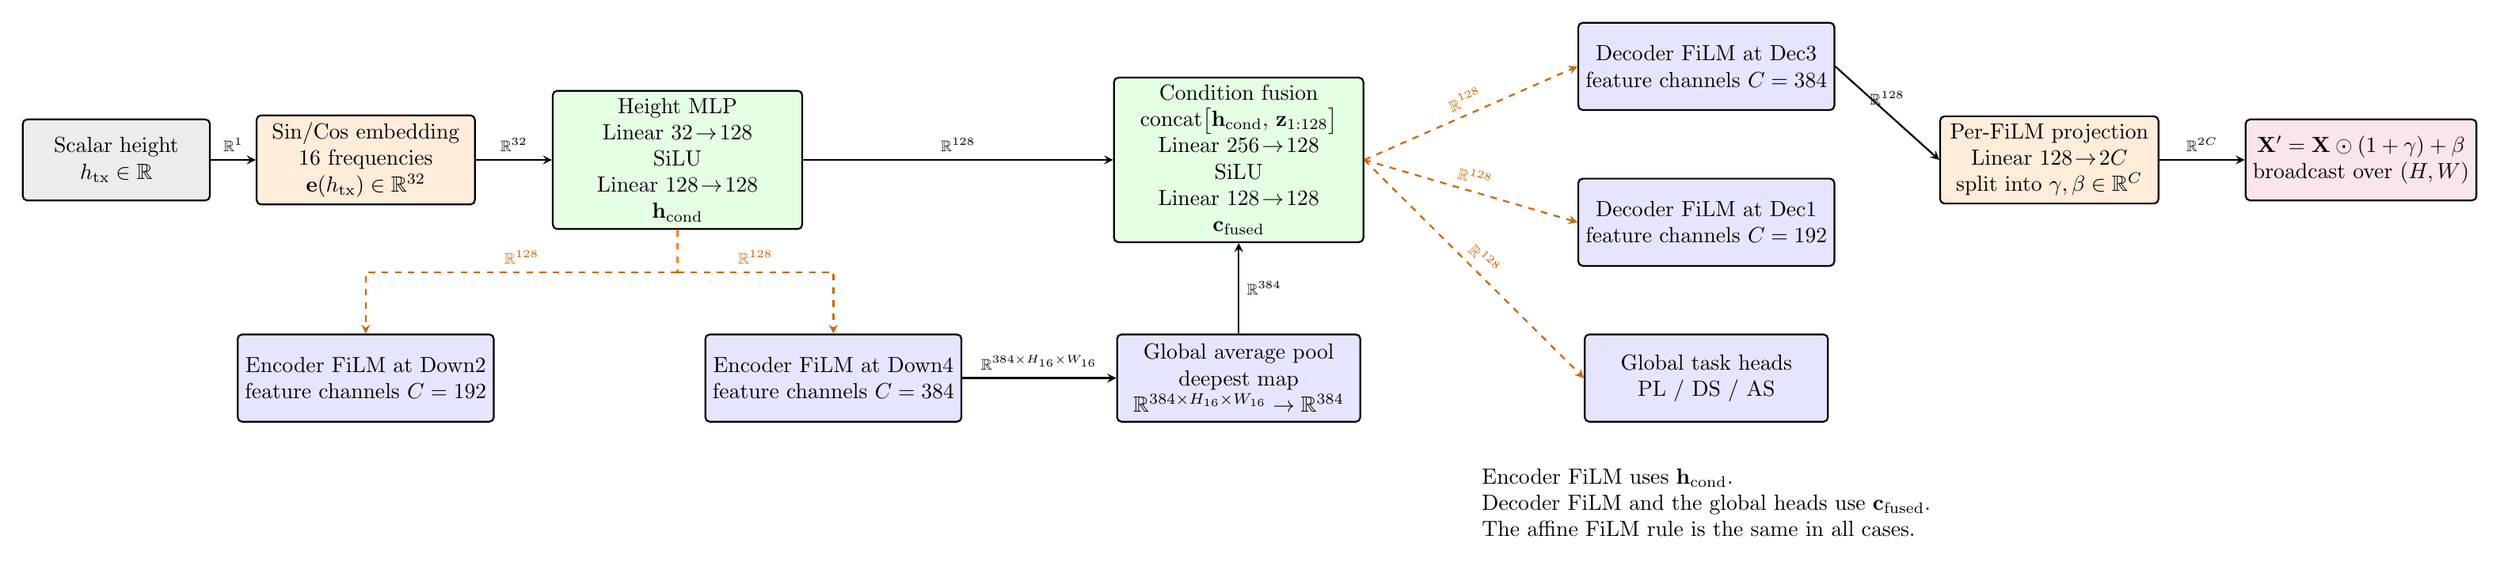
\begin{tikzpicture}[
    >=stealth,
    font=\normalsize,
    smallbox/.style={draw, thick, rounded corners=2pt, rectangle, minimum width=3.0cm, minimum height=1.3cm, align=center},
    opbox/.style={draw, thick, rounded corners=2pt, rectangle, minimum width=3.5cm, minimum height=1.4cm, align=center, fill=orange!15},
    featbox/.style={draw, thick, rounded corners=2pt, rectangle, minimum width=3.9cm, minimum height=1.4cm, align=center, fill=blue!10},
    condbox/.style={draw, thick, rounded corners=2pt, rectangle, minimum width=4.0cm, minimum height=1.4cm, align=center, fill=green!10},
    note/.style={font=\normalsize, align=left},
    arr/.style={->, thick},
    condarr/.style={->, thick, orange!80!black, dashed}
]

\node[smallbox, fill=gray!15] (h) at (0,0) {Scalar height\\$h_{\mathrm{tx}} \in \mathbb{R}$};
\node[opbox] (embed) at (4.0,0) {Sin/Cos embedding\\16 frequencies\\$\mathbf{e}(h_{\mathrm{tx}})\in\mathbb{R}^{32}$};
\node[condbox] (mlp1) at (9.0,0) {Height MLP\\Linear $32\!\to\!128$\\SiLU\\Linear $128\!\to\!128$\\$\mathbf{h}_{\mathrm{cond}}$};

\draw[arr] (h) -- node[above, font=\scriptsize] {$\mathbb{R}^{1}$} (embed);
\draw[arr] (embed) -- node[above, font=\scriptsize] {$\mathbb{R}^{32}$} (mlp1);

\node[featbox] (enc2) at (4.0,-3.5) {Encoder FiLM at Down2\\feature channels $C=192$};
\node[featbox] (enc4) at (11.5,-3.5) {Encoder FiLM at Down4\\feature channels $C=384$};
\draw[thick, orange, dashed] (mlp1.south) -- (9.0, -1.8);
\draw[condarr] (9.0, -1.8) -- node[above, font=\scriptsize] {$\mathbb{R}^{128}$} (4.0, -1.8) -- (enc2.north);
\draw[condarr] (9.0, -1.8) -- node[above, font=\scriptsize] {$\mathbb{R}^{128}$} (11.5, -1.8) -- (enc4.north);

\node[featbox] (pool) at (18.0,-3.5) {Global average pool\\deepest map\\$\mathbb{R}^{384\times H_{16}\times W_{16}} \to \mathbb{R}^{384}$};
\draw[arr] (enc4.east) -- node[above, font=\scriptsize] {$\mathbb{R}^{384\times H_{16}\times W_{16}}$} (pool.west);

\node[condbox] (fuse) at (18.0,0) {Condition fusion\\concat$\bigl[\mathbf{h}_{\mathrm{cond}},\,\mathbf{z}_{1:128}\bigr]$\\Linear $256\!\to\!128$\\SiLU\\Linear $128\!\to\!128$\\$\mathbf{c}_{\mathrm{fused}}$};
\draw[arr] (mlp1.east) -- node[above, font=\scriptsize] {$\mathbb{R}^{128}$} (fuse.west);
\draw[arr] (pool.north) -- node[right, font=\scriptsize] {$\mathbb{R}^{384}$} (fuse.south);

\node[featbox] (dec3) at (25.5, 1.5) {Decoder FiLM at Dec3\\feature channels $C=384$};
\node[featbox] (dec1) at (25.5,-1.0) {Decoder FiLM at Dec1\\feature channels $C=192$};
\node[featbox] (gh) at (25.5,-3.5) {Global task heads\\PL / DS / AS};
\draw[condarr] (fuse.east) -- node[above, sloped, font=\scriptsize] {$\mathbb{R}^{128}$} (dec3.west);
\draw[condarr] (fuse.east) -- node[above, sloped, font=\scriptsize] {$\mathbb{R}^{128}$} (dec1.west);
\draw[condarr] (fuse.east) -- node[above, sloped, font=\scriptsize] {$\mathbb{R}^{128}$} (gh.west);

\node[opbox] (filmproj) at (31.0,0.0) {Per-FiLM projection\\Linear $128\!\to\!2C$\\split into $\gamma,\beta \in \mathbb{R}^{C}$};
\node[smallbox, fill=purple!10] (affine) at (36.0,0.0) {$\mathbf{X}'=\mathbf{X}\odot(1+\gamma)+\beta$\\broadcast over $(H,W)$};
\draw[arr] (dec3.east) -- node[above, font=\scriptsize] {$\mathbb{R}^{128}$} (filmproj.west);
\draw[arr] (filmproj.east) -- node[above, font=\scriptsize] {$\mathbb{R}^{2C}$} (affine.west);

\node[note] at (25.5,-5.5) {Encoder FiLM uses $\mathbf{h}_{\mathrm{cond}}$.\\Decoder FiLM and the global heads use $\mathbf{c}_{\mathrm{fused}}$.\\The affine FiLM rule is the same in all cases.};

\end{tikzpicture}%
}
\caption{Detailed \texttt{Try 80} sinusoidal height-conditioning path. The scalar
UAV height is encoded by a 32-dimensional sinusoidal embedding, lifted to
$\mathbf{h}_{\mathrm{cond}} \in \mathbb{R}^{128}$, and used to FiLM-modulate
the encoder. After pooling the deepest map, a fused condition
$\mathbf{c}_{\mathrm{fused}}$ is built and reused by decoder FiLM layers and
the global task heads.}
\label{fig:try80_film_detail}
\end{figure}

\paragraph{Detailed prior-anchored GMM head.}
The actual GMM assembly is also more structured than the compact summary in
Figure~\ref{fig:try80_arch}. For each task
$k \in \{\mathrm{PL},\mathrm{DS},\mathrm{AS}\}$ and for each region
$r \in \{\mathrm{LoS},\mathrm{NLoS}\}$, the model predicts a 3-component
mixture. The global head outputs
$\pi^{(g)}_{k,r,j}$, $\delta^{(g)}_{k,r,j}$ and $\sigma^{(g)}_{k,r,j}$, while
the local head outputs per-pixel maps
$p^{(\ell)}_{k,r,j}(x)$, $\delta^{(\ell)}_{k,r}(x)$, $\alpha_{k,r}(x)$, and
$\tilde\sigma_{k,r}(x)$. In code, these are transformed as
\begin{align}
\pi_{k,r,j} &= \mathrm{softmax}\!\left(\mathrm{pi\_logits}_{k,r,\cdot}\right)_j \\
p_{k,r,j}(x) &= \mathrm{softmax}\!\left(\mathrm{p\_logits}_{k,r,\cdot}(x)\right)_j \\
\delta^{(g)}_{k,r,j} &= \tanh\!\left(\delta^{(g),\mathrm{raw}}_{k,r,j}\right)\,\delta_{\max,k,r} \\
\delta^{(\ell)}_{k,r}(x) &= \tanh\!\left(\delta^{(\ell),\mathrm{raw}}_{k,r}(x)\right)\,\delta_{\max,k,r} \\
\alpha_{k,r}(x) &= \sigma\!\left(\alpha^{\mathrm{raw}}_{k,r}(x) - 2\right) \\
\sigma^{(g)}_{k,r,j} &= \sigma_{\min} + \sigma\!\left(s^{(g),\mathrm{raw}}_{k,r,j}\right)\left(\sigma_{\max}-\sigma_{\min}\right) \\
\tilde\sigma_{k,r}(x) &= \sigma_{\min} + \sigma\!\left(\tilde s^{\mathrm{raw}}_{k,r}(x)\right)\left(\sigma_{\max}-\sigma_{\min}\right)
\end{align}
with $\sigma_{\min}=0.05$ and $\sigma_{\max}=3.0$ in the default
configuration. The final component parameters are
\begin{align}
\Delta_{k,r,j}(x) &= \mathrm{clip}\!\left(\delta^{(g)}_{k,r,j} + \delta^{(\ell)}_{k,r}(x),\,
[-\delta_{\max,k,r}, +\delta_{\max,k,r}]\right) \\
\mu_{k,r,j}(x) &= y^{\mathrm{prior}}_{k,r}(x) + \alpha_{k,r}(x)\,\Delta_{k,r,j}(x) \\
\sigma_{k,r,j}(x) &= \sqrt{\left(\sigma^{(g)}_{k,r,j}\right)^2 + \left(\tilde\sigma_{k,r}(x)\right)^2}
\label{eq:try80_sigma_detail}
\end{align}
For path loss, this is already the transformed training space because path loss
is trained directly in dB. For delay spread and angular spread, the residual
cap and the anchored mean are defined in native units first, and the resulting
mean is then mapped through $\log(1+\cdot)$ before evaluating the Gaussian NLL.
and the regional deterministic prediction becomes
\begin{equation}
\hat y_{k,r}(x) = \sum_{j=1}^{3} p_{k,r,j}(x)\,\mu_{k,r,j}(x)
\label{eq:try80_region_point}
\end{equation}
after which the final map uses the explicit LoS/NLoS masks to select the
appropriate regional prediction at each pixel.
The quantities $\delta_{\max,k,r}$ are not additional GMM outputs. They are
fixed task- and region-specific safety caps that define how far the learned
residual is allowed to move away from the frozen prior. Conceptually, the caps
used for the three native targets are:
\begin{equation}
\delta_{\max,k,r}
=
\begin{cases}
2~\mathrm{dB}, & k=\mathrm{PL},\ r=\mathrm{LoS},\\
4~\mathrm{dB}, & k=\mathrm{PL},\ r=\mathrm{NLoS},\\
30, & k=\mathrm{DS},\ r=\mathrm{LoS},\\
40, & k=\mathrm{DS},\ r=\mathrm{NLoS},\\
9, & k=\mathrm{AS},\ r=\mathrm{LoS},\\
13, & k=\mathrm{AS},\ r=\mathrm{NLoS}.
\end{cases}
\label{eq:try80_native_residual_caps}
\end{equation}
The larger NLoS caps reflect the higher uncertainty and stronger residual
structure in obstructed pixels.

\begin{figure}[H]
\centering
\resizebox{\textwidth}{!}{%
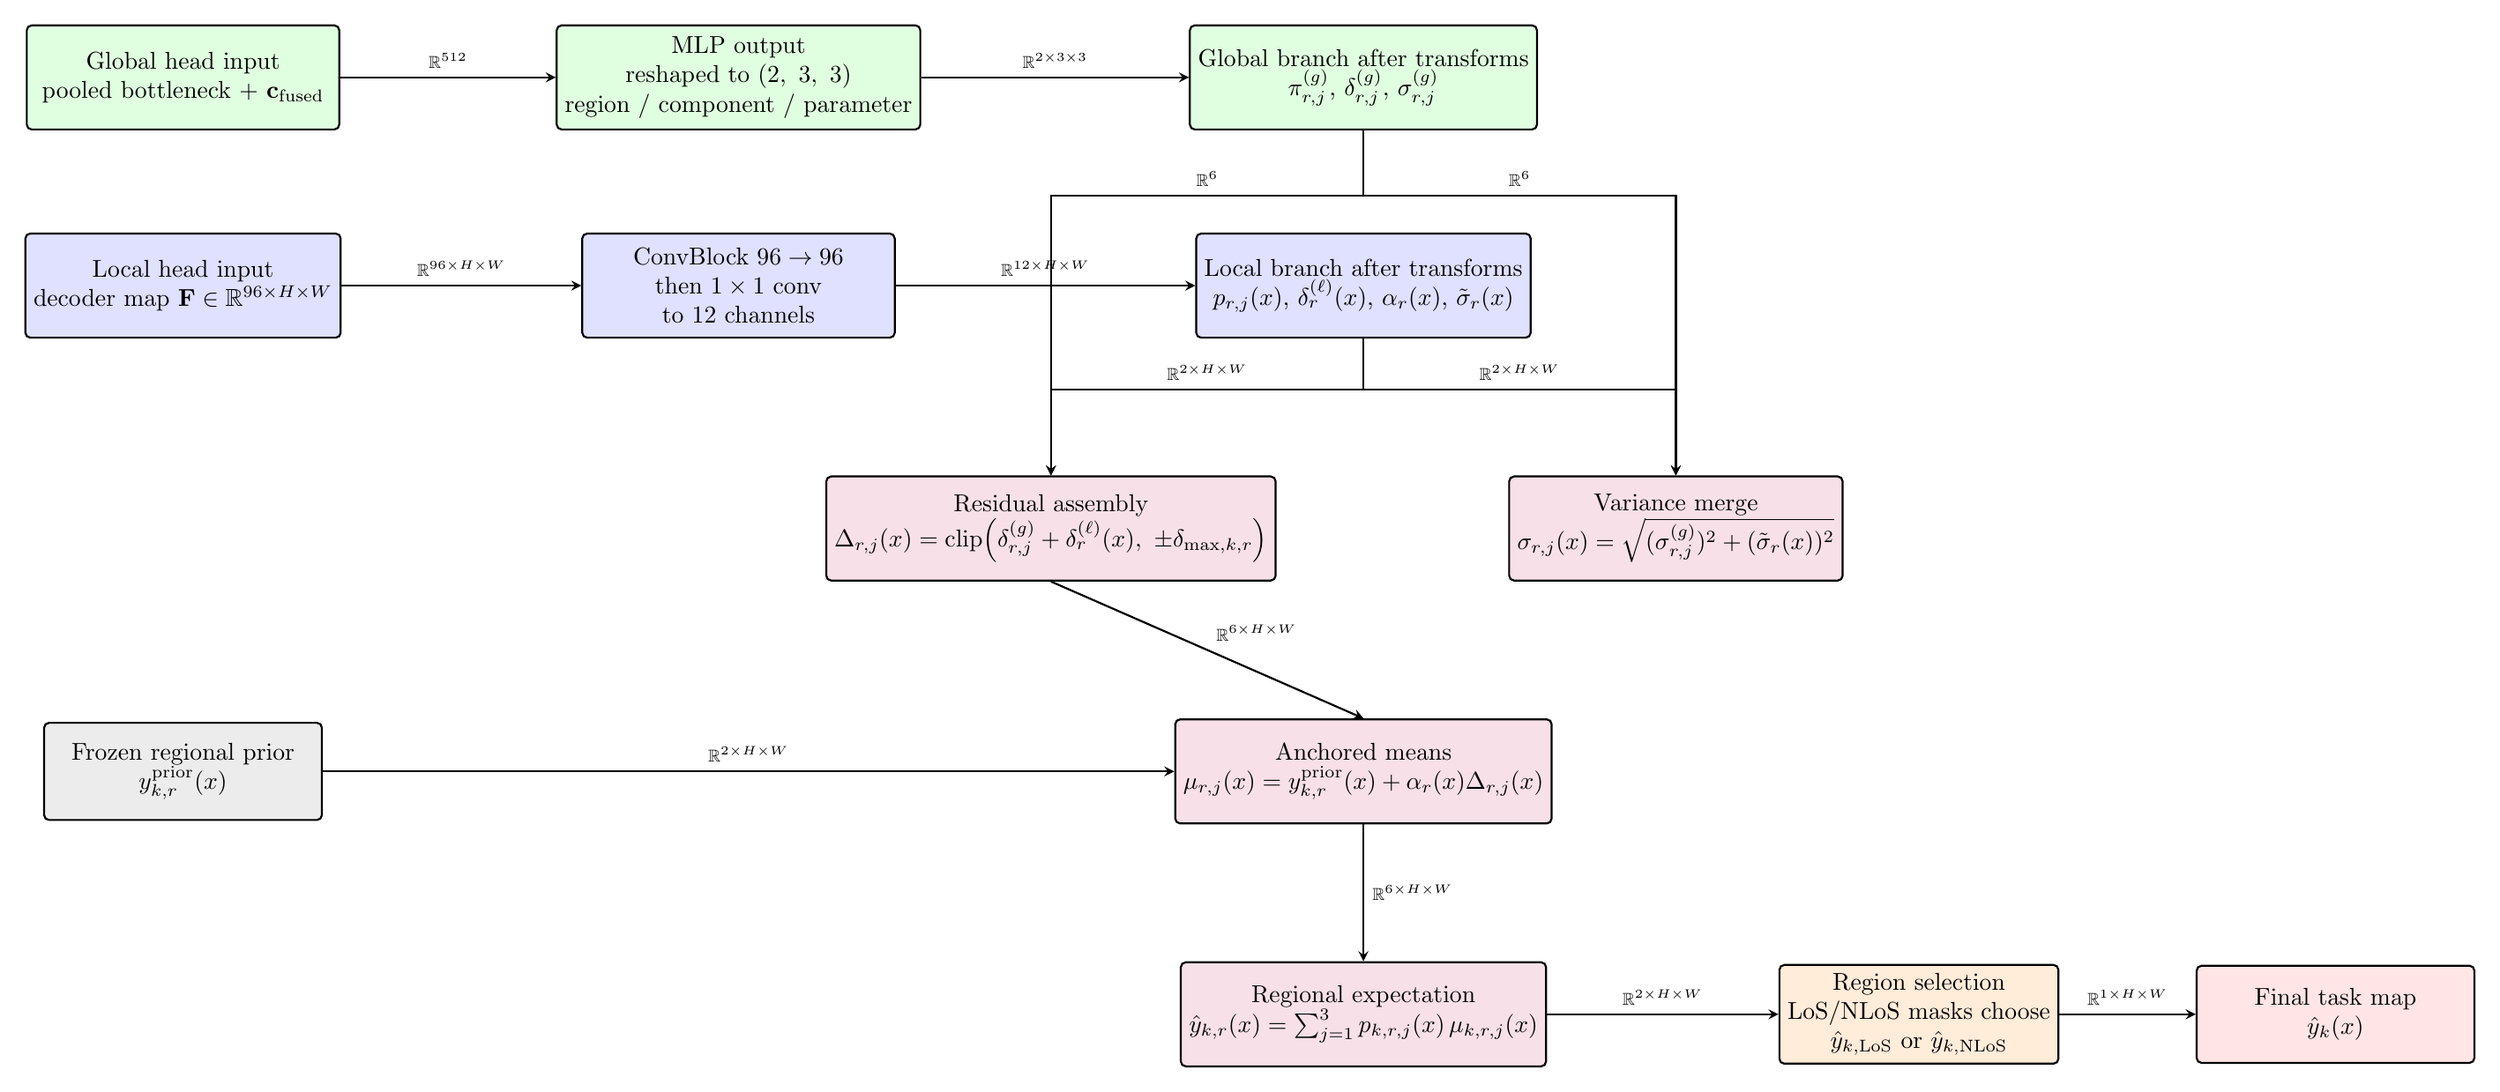
\begin{tikzpicture}[
    >=stealth,
    font=\normalsize,
    box/.style={draw, thick, rounded corners=2pt, rectangle, minimum width=4.0cm, minimum height=1.4cm, align=center},
    prior/.style={draw, thick, rounded corners=2pt, rectangle, minimum width=4.0cm, minimum height=1.4cm, align=center, fill=gray!15},
    global/.style={draw, thick, rounded corners=2pt, rectangle, minimum width=4.5cm, minimum height=1.5cm, align=center, fill=green!12},
    local/.style={draw, thick, rounded corners=2pt, rectangle, minimum width=4.5cm, minimum height=1.5cm, align=center, fill=blue!12},
    mix/.style={draw, thick, rounded corners=2pt, rectangle, minimum width=4.8cm, minimum height=1.5cm, align=center, fill=purple!12},
    arr/.style={->, thick}
]

\node[global] (globin) at (0,3.5) {Global head input\\pooled bottleneck $+\ \mathbf{c}_{\mathrm{fused}}$};
\node[global] (globraw) at (8.0,3.5) {MLP output\\reshaped to $(2,\ 3,\ 3)$\\region / component / parameter};
\node[global] (globpars) at (17.0,3.5) {Global branch after transforms\\$\pi^{(g)}_{r,j}$, $\delta^{(g)}_{r,j}$, $\sigma^{(g)}_{r,j}$};
\draw[arr] (globin) -- node[above, font=\scriptsize] {$\mathbb{R}^{512}$} (globraw);
\draw[arr] (globraw) -- node[above, font=\scriptsize] {$\mathbb{R}^{2 \times 3 \times 3}$} (globpars);

\node[local] (locin) at (0,0.5) {Local head input\\decoder map $\mathbf{F}\in\mathbb{R}^{96\times H\times W}$};
\node[local] (locraw) at (8.0,0.5) {ConvBlock $96\to96$\\then $1\times1$ conv\\to 12 channels};
\node[local] (locpars) at (17.0,0.5) {Local branch after transforms\\$p_{r,j}(x)$, $\delta^{(\ell)}_{r}(x)$, $\alpha_r(x)$, $\tilde\sigma_r(x)$};
\draw[arr] (locin) -- node[above, font=\scriptsize] {$\mathbb{R}^{96 \times H \times W}$} (locraw);
\draw[arr] (locraw) -- node[above, font=\scriptsize] {$\mathbb{R}^{12 \times H \times W}$} (locpars);

\node[mix] (delta) at (12.5,-3.0) {Residual assembly\\$\Delta_{r,j}(x)=\mathrm{clip}\!\left(\delta^{(g)}_{r,j}+\delta^{(\ell)}_{r}(x),\ \pm\delta_{\max,k,r}\right)$};
\node[prior] (prior) at (0,-6.5) {Frozen regional prior\\$y^{\mathrm{prior}}_{k,r}(x)$};
\node[mix] (mu) at (17.0,-6.5) {Anchored means\\$\mu_{r,j}(x)=y^{\mathrm{prior}}_{k,r}(x)+\alpha_r(x)\Delta_{r,j}(x)$};
\node[mix] (sigma) at (21.5,-3.0) {Variance merge\\$\sigma_{r,j}(x)=\sqrt{(\sigma^{(g)}_{r,j})^2+(\tilde\sigma_r(x))^2}$};

\draw[thick] (globpars.south) -- (17.0, 1.8);
\draw[arr] (17.0, 1.8) -- node[above, font=\scriptsize] {$\mathbb{R}^{6}$} (12.5, 1.8) -- (delta.north);
\draw[arr] (17.0, 1.8) -- node[above, font=\scriptsize] {$\mathbb{R}^{6}$} (21.5, 1.8) -- (sigma.north);

\draw[thick] (locpars.south) -- (17.0, -1.0);
\draw[arr] (17.0, -1.0) -- node[above, font=\scriptsize] {$\mathbb{R}^{2 \times H \times W}$} (12.5, -1.0) -- (delta.north);
\draw[arr] (17.0, -1.0) -- node[above, font=\scriptsize] {$\mathbb{R}^{2 \times H \times W}$} (21.5, -1.0) -- (sigma.north);

\draw[arr] (delta.south) -- node[above right, font=\scriptsize] {$\mathbb{R}^{6 \times H \times W}$} (mu.north);
\draw[arr] (prior.east) -- node[above, font=\scriptsize] {$\mathbb{R}^{2 \times H \times W}$} (mu.west);

\node[mix] (expv) at (17.0,-10.0) {Regional expectation\\$\hat y_{k,r}(x)=\sum_{j=1}^{3} p_{k,r,j}(x)\,\mu_{k,r,j}(x)$};
\node[box, fill=orange!15] (mask) at (25.0,-10.0) {Region selection\\LoS/NLoS masks choose\\$\hat y_{k,\mathrm{LoS}}$ or $\hat y_{k,\mathrm{NLoS}}$};
\node[box, fill=red!10] (out) at (31.0,-10.0) {Final task map\\$\hat y_k(x)$};

\draw[arr] (mu.south) -- node[right, font=\scriptsize] {$\mathbb{R}^{6 \times H \times W}$} (expv.north);
\draw[arr] (expv.east) -- node[above, font=\scriptsize] {$\mathbb{R}^{2 \times H \times W}$} (mask.west);
\draw[arr] (mask.east) -- node[above, font=\scriptsize] {$\mathbb{R}^{1 \times H \times W}$} (out.west);

\end{tikzpicture}%
}
\caption{Detailed prior-anchored GMM head used by \texttt{Try 80} for each task (path loss, delay spread or angular spread).
Each task predicts separate LoS and NLoS 3-component mixtures. The global head
produces map-level mixture structure, the local head produces pixelwise
refinements, and both are combined around the frozen prior under explicit
residual caps.}
\label{fig:try80_gmm_detail}
\end{figure}

\subsubsection{Composite Optimization Objective}

Equation~\ref{eq:try80_loss} highlights the core philosophy, but the actual implementation utilizes a robust composite loss to stabilize the GMM training and prevent mode collapse:

\begin{itemize}
\item \textbf{Negative Log-Likelihood ($\mathcal{L}_{\mathrm{NLL}}$)}: The primary data-fidelity term, computed under the predicted GMM and evaluated independently for LoS and NLoS regions using explicit region masks.
\item \textbf{Prior Guard ($\mathcal{L}_{\mathrm{guard}}$)}: The asymmetric penalty (Eq.~\ref{eq:try80_loss}) that penalizes the network strictly on pixels where its squared error exceeds that of the deterministic physical prior.
\item \textbf{Anchor Penalty ($\mathcal{L}_{\mathrm{anchor}}$)}: Direct L2 regularization on $\alpha_k(x)$, $\delta_{\mathrm{global}}$, and $\delta_{\mathrm{local}}$. This mathematically anchors the network to the physical priors, forcing the deep learning layers to ''justify'' any deviations.
\item \textbf{Distributional KL-Divergence ($\mathcal{L}_{\mathrm{KL}}$)}: A soft-histogram loss that encourages the marginal distribution of the predicted GMM to match the empirical distribution of residuals in the current batch.
\item \textbf{Outlier Budget}: A penalty that bounds the probability mass assigned to the third GMM component (designed for severe multipath outliers), preventing it from indiscriminately absorbing general variance.
\item \textbf{Moment Matching \& Auxiliary Losses}: Includes RMSE, MAE, and spatial moment-matching (penalizing differences in map mean and variance) applied directly to the deterministic expected value $\hat y_k(x)$ to accelerate early-stage convergence.
\end{itemize}

%% ============================================================
\section{Limitations and validity considerations}
%% ============================================================

The hybrid design is intentionally more interpretable than a purely black-box
model, but the following limitations should be stated explicitly:

\begin{itemize}
\item \textbf{The priors are calibrated to CKM.}
      The fitted two-ray parameters, morphology coefficients and ridge
      coefficients are not universal propagation constants. They are
      dataset-calibrated parameters for the CKM map distribution and split.

\item \textbf{COST-231 is used outside its original validation regime.}
      In this work it serves as a coarse NLoS envelope, not as a claim that
      terrestrial COST-231/Hata is directly valid for all UAV heights.

\item \textbf{The LoS/NLoS mask is a geometric dataset signal.}
      \texttt{Try 80} uses explicit LoS and NLoS masks produced from the CKM
      geometry. This is appropriate for the current map-based setting, but it
      should be described as a geometry-informed model rather than a model that
      infers LoS/NLoS from raw measurements alone.

\item \textbf{The GMM is predictive, not a full 3GPP channel simulator.}
      The mixture describes uncertainty and residual modes of the map target at
      each pixel. It does not generate a complete stochastic multipath channel
      realization with delays, angles, cluster powers and temporal evolution.

\item \textbf{Final \texttt{Try 80} claims require a frozen checkpoint.}
      Since the full training is still ongoing, any final comparison against
      the frozen priors or previous deep models should be made only after the
      selected checkpoint, validation criterion and held-out test evaluation
      are fixed.
\end{itemize}

Recommended ablations for the final report are: frozen prior only,
\texttt{Try 80} without the prior guard, without residual caps, without
multi-task sharing, without FiLM height conditioning, and with deterministic
regression losses instead of the prior-anchored GMM head.

%% ============================================================
\section{Why these changes were made}
%% ============================================================

\begin{enumerate}
\item \textbf{The CKM maps show strong dataset-specific structure.}
      In particular, LoS path loss showed ring-like residual behavior around
      the transmitter, which justified a fitted two-ray treatment instead of a
      generic uncalibrated model.

\item \textbf{The task is pixel-map prediction, not only scenario-level modeling.}
      Classical channel models are usually written for statistical scenario
      simulation, whereas here the aim is to predict a full spatial field over
      a map.

\item \textbf{Interpretability was intentionally preserved.}
      Both \texttt{Try 78} and \texttt{Try 79} remain readable and
      coefficient-level inspectable. This makes them useful as thesis material
      and as robust baselines.

\item \textbf{Deep learning was introduced only after the priors were strong.}
      The philosophy in \texttt{Try 80} is that deep learning should model the
      residual uncertainty, not replace known deterministic structure.
\end{enumerate}

%% ============================================================
\section{Summary}
%% ============================================================

\begin{quote}
The literature provided the physical and statistical starting points
(two-ray LoS behavior, coarse urban path-loss envelopes, log-domain treatment
of delay/angular spreads, and LoS/NLoS regime separation). The actual work was
to adapt those ideas to the CKM map setting, calibrate them with map-derived
features, and then integrate them into a single residual multi-task deep model
in \texttt{Try 80}. The calibration methodology was: grid search over the
two-ray parameters $(\rho, \phi)$ for the LoS branch, followed by Gaussian
post-smoothing; regime-wise linear calibration over 15 morphology/geometry
features for the path-loss branch; and ridge regression with
$\lambda = 10^{-3}$ over 23 morphology/geometry features for the spread
branches. Therefore, the novelty is not ``inventing a new textbook propagation
law'', but building a practical hybrid pipeline that is both interpretable and
trainable on the dataset at hand. The final quantitative claims for
\texttt{Try 80} itself should be added only after the ongoing training run has
finished and a checkpoint has been selected.
\end{quote}

%% ============================================================
\clearpage
\section{Sources}
%% ============================================================

\subsection{Project sources}
\small
\begin{itemize}
\item \textbf{Try 80 integration code:}
      \texttt{TFGEightiethTry80/src/priors\_try80.py}.

\item \textbf{Try 80 design note:}
      \texttt{TFGEightiethTry80/DESIGN\_TRY80.md}.

\item \textbf{Try 80 model and loss implementation:}
      \texttt{TFGEightiethTry80/src/model\_try80.py} and
      \texttt{TFGEightiethTry80/src/losses\_try80.py}.

\item \textbf{Try 80 resolved training configuration:}
      \texttt{cluster\_outputs/TFGEightiethTry80/try80\_joint\_big/resolved\_config.json}.

\item \textbf{Try 78 final result file:}
      \texttt{TFGSeventyEighthTry78/hybrid\_out\_final\_dml/hybrid\_eval\_summary.json}.

\item \textbf{Try 79 final test result file:}
      \texttt{TFGSeventyNinthTry79/test\_eval\_dml\_hz\_v2/eval\_summary\_test.json}.

\item \textbf{Try 79 calibration file:}
      \texttt{TFGSeventyNinthTry79/test\_eval\_dml\_hz\_v2/calibration.json}.

\item \textbf{Try 78 interpretation note:}
      \texttt{TFGSeventyEighthTry78/TRY78\_LOS\_DOCUMENTATION.md}.

\item \textbf{Try 79 interpretation note:}
      \texttt{TFGSeventyNinthTry79/README.md}.
\end{itemize}
\normalsize
\subsection{Literature sources}

\begin{thebibliography}{99}

\bibitem{tr38901}
3GPP TR 38.901,
\emph{Study on Channel Model for Frequencies from 0.5 to 100 GHz}.
\url{https://www.3gpp.org/ftp/Specs/archive/38_series/38.901/}

\bibitem{winner2}
P. Ky\"osti et al.,
\emph{WINNER II Channel Models},
IST-4-027756 WINNER II Deliverable.
\url{https://www.ist-winner.org/WINNER2-Deliverables/D1.1.2v1.2.pdf}

\bibitem{wocc2021}
Y.-S. Su, S.-C. Lin, and K.-C. Chen,
``Channel Modeling of Air-to-Ground Signal with Two-Ray Model at Low-Altitude Platforms,''
in \emph{Proc. WOCC}, 2021.
\url{https://doi.org/10.1109/WOCC53213.2021.9603250}

\bibitem{khawaja_survey}
W. Khawaja, I. Guvenc, D. Matolak, U.-C. Fiebig, and N. Schneckenberger,
``A Survey of Air-to-Ground Propagation Channel Modeling for Unmanned Aerial Vehicles,''
\emph{arXiv preprint arXiv:1801.01656}, 2018.
\url{https://arxiv.org/abs/1801.01656}

\bibitem{cai2019}
X. Cai, J. Rodr\'iguez-Pi\~neiro, X. Yin, B. Ai, G. F. Pedersen, and A. Perez Yuste,
``An Empirical Air-to-Ground Channel Model Based on Passive Measurements in LTE,''
\emph{arXiv preprint arXiv:1901.07930}, 2019.
\url{https://arxiv.org/abs/1901.07930}

\bibitem{izydorczyk2019}
T. Izydorczyk, F. M. L. Tavares, G. Berardinelli, M. Bucur, and P. Mogensen,
``Angular Distribution of Cellular Signals for UAVs in Urban and Rural Scenarios,''
in \emph{Proc. EuCAP}, 2019.
\url{https://vbn.aau.dk/ws/files/306998488/Angular_Distribution_of_Cellular_Signals_for_UAVs_in_Urban_and_Rural_Scenarios.pdf}

\bibitem{rappaport}
T. S. Rappaport,
\emph{Wireless Communications: Principles and Practice}.
Prentice Hall.
\url{https://search.worldcat.org/es/title/Wireless-communications-%3A-principles-and-practice/oclc/318358858}

\end{thebibliography}

\end{document}
